\documentclass{ws-ijbc}

%%%%%%%%%%%%%%%%
% Instructions %
%%%%%%%%%%%%%%%%
% Set the document class and settings to match the final document that these figures_raw will be included into
% This will output a pdf with a page for each figure, nicely cropped according to picture dimenstions as defined below in the `Figure' Section. Inlcude in the final document by using package 'graphicx' and command \includegraphics[page=<page of figure>]{figures_raw.pdf}
% The following package is used to create the cropping mentioned above, and apparently should be the last loaded package: \usepackage[active,tightpage]{preview}
% The following command re-writes the figure enviroment to become a preview enviroment - without this spacing is off, and captions and labels may appear
%\renewenvironment{figure}[1][]{%
%	\begin{preview}%
%		\renewcommand{\caption}[2][]{}}
%	{\end{preview}}

%%%%%%%%%%%%%%%%%
% Load Packages %
%%%%%%%%%%%%%%%%%
\usepackage{epsfig}
\usepackage{amssymb}
\pagestyle{empty}
\usepackage{epstopdf}
\usepackage{mathrsfs}
\usepackage{amsmath}
\usepackage{graphicx}
\usepackage{array}
\usepackage{xcolor}    % \nopagecolor
\usepackage{fp}
\usepackage[T1]{fontenc}
\usepackage{bm}    % boldmath \bm{}
\usepackage[pdftex,active,tightpage]{preview}    % should be loaded lasts
% adjust borders added to figures_raw: left, lower, right and upper borders. - useful to increase lower border not to cut off labels placed below figure bounds. 
\renewcommand{\PreviewBbAdjust}{0mm -0.25mm 0mm 0mm}
\renewenvironment{figure}[1][]{%
	\begin{preview}%
		\renewcommand{\caption}[2][]{}}
	{\end{preview}}

\setlength{\unitlength}{1mm}

%%%%%%%%%%%%%%%%%%%%%%%%%%%%%%%%%%%%%%%%%%%%%%%%
% Get various dimensions for the documentclass %
%%%%%%%%%%%%%%%%%%%%%%%%%%%%%%%%%%%%%%%%%%%%%%%%
\makeatletter
\newcommand*{\getlength}[1]{\strip@pt\dimexpr0.035136\dimexpr#1\relax\relax}
\newcommand{\showfont}{%
encoding: \f@encoding{},\\
family: \f@family{},\\
series: \f@series{},\\
shape: \f@shape{},\\
size: \f@size{} pt,\\
text height: \getlength{\the\textheight} cm,\\
text width:     \getlength{\the\textwidth} cm}
\makeatother

\begin{document}
%\begin{figure}
%	\begin{picture}(20,5)(0,0)
%		\showfont
%	\end{picture}
%\end{figure}
%\newpage
%%%%%%%%%%%%%%%%
%%% Figure 1: Critical manifold %%%
%%%%%%%%%%%%%%%%
\nopagecolor
\begin{figure}
	\begin{picture}(85,44)(5.5,6.5)
	\put(10.25,10){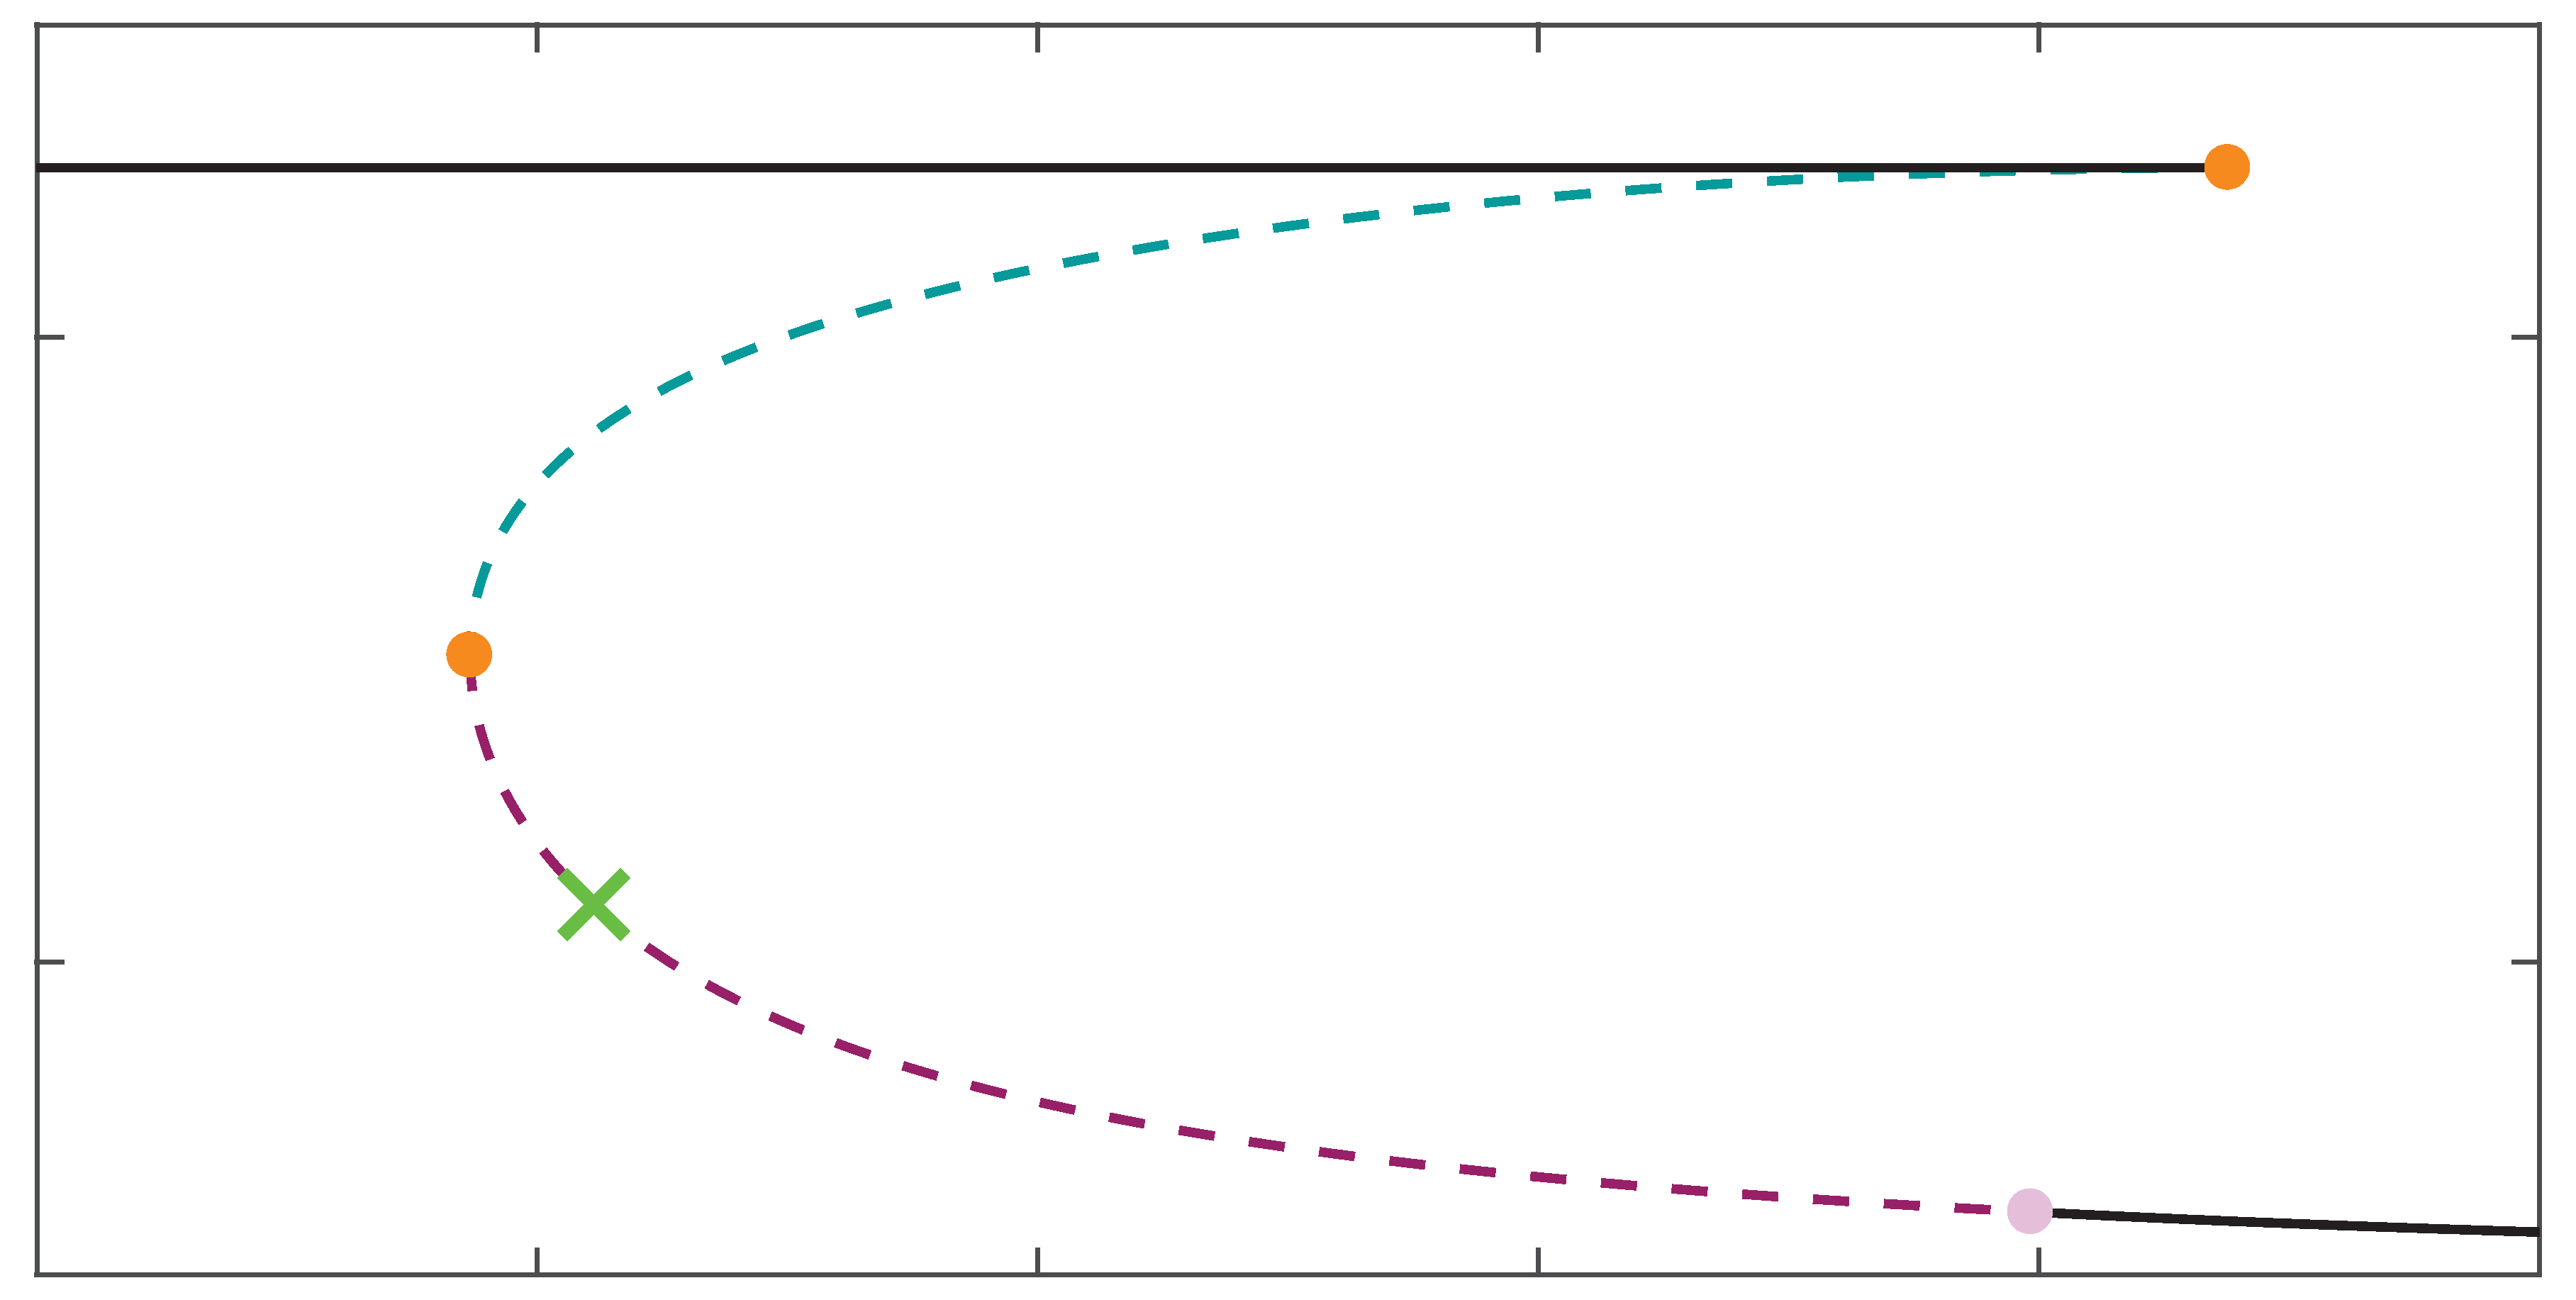
\includegraphics[width=8cm]{./figures_raw/paper_critical.eps}}
	\put(81,44){$F_1$}
        \put(19,29){$F_2$}
        \put(72.5,13.5){$H$}
        \put(80,13){$C^4_-$}
        \put(20,41.5){$C^4_+$}
        \put(50,40){$C^3$}
        \put(50,15){$C^2$}
        \put(7,46){$A$}
        \put(6,39){\footnotesize $9.0$}
        \put(6,19){\footnotesize $3.0$}
	\put(24.5,7.5){\footnotesize $0.3$}
	\put(40.4,7.5){\footnotesize $0.5$}
	\put(56.4,7.5){\footnotesize $0.7$}
	\put(72.2,7.5){\footnotesize $0.9$}
	\put(86,6.9){$B$}
	\put(25,20){$q$}
	\end{picture}
	\caption{}
\end{figure}
\newpage

%%%%%%%%%%%%%%%%%%
%%%% Figure 2: Tube figure %%%
%%%%%%%%%%%%%%%%%%

\begin{figure}
	\begin{picture}(114.75,63)(94.75,97)
	    \put(100,100){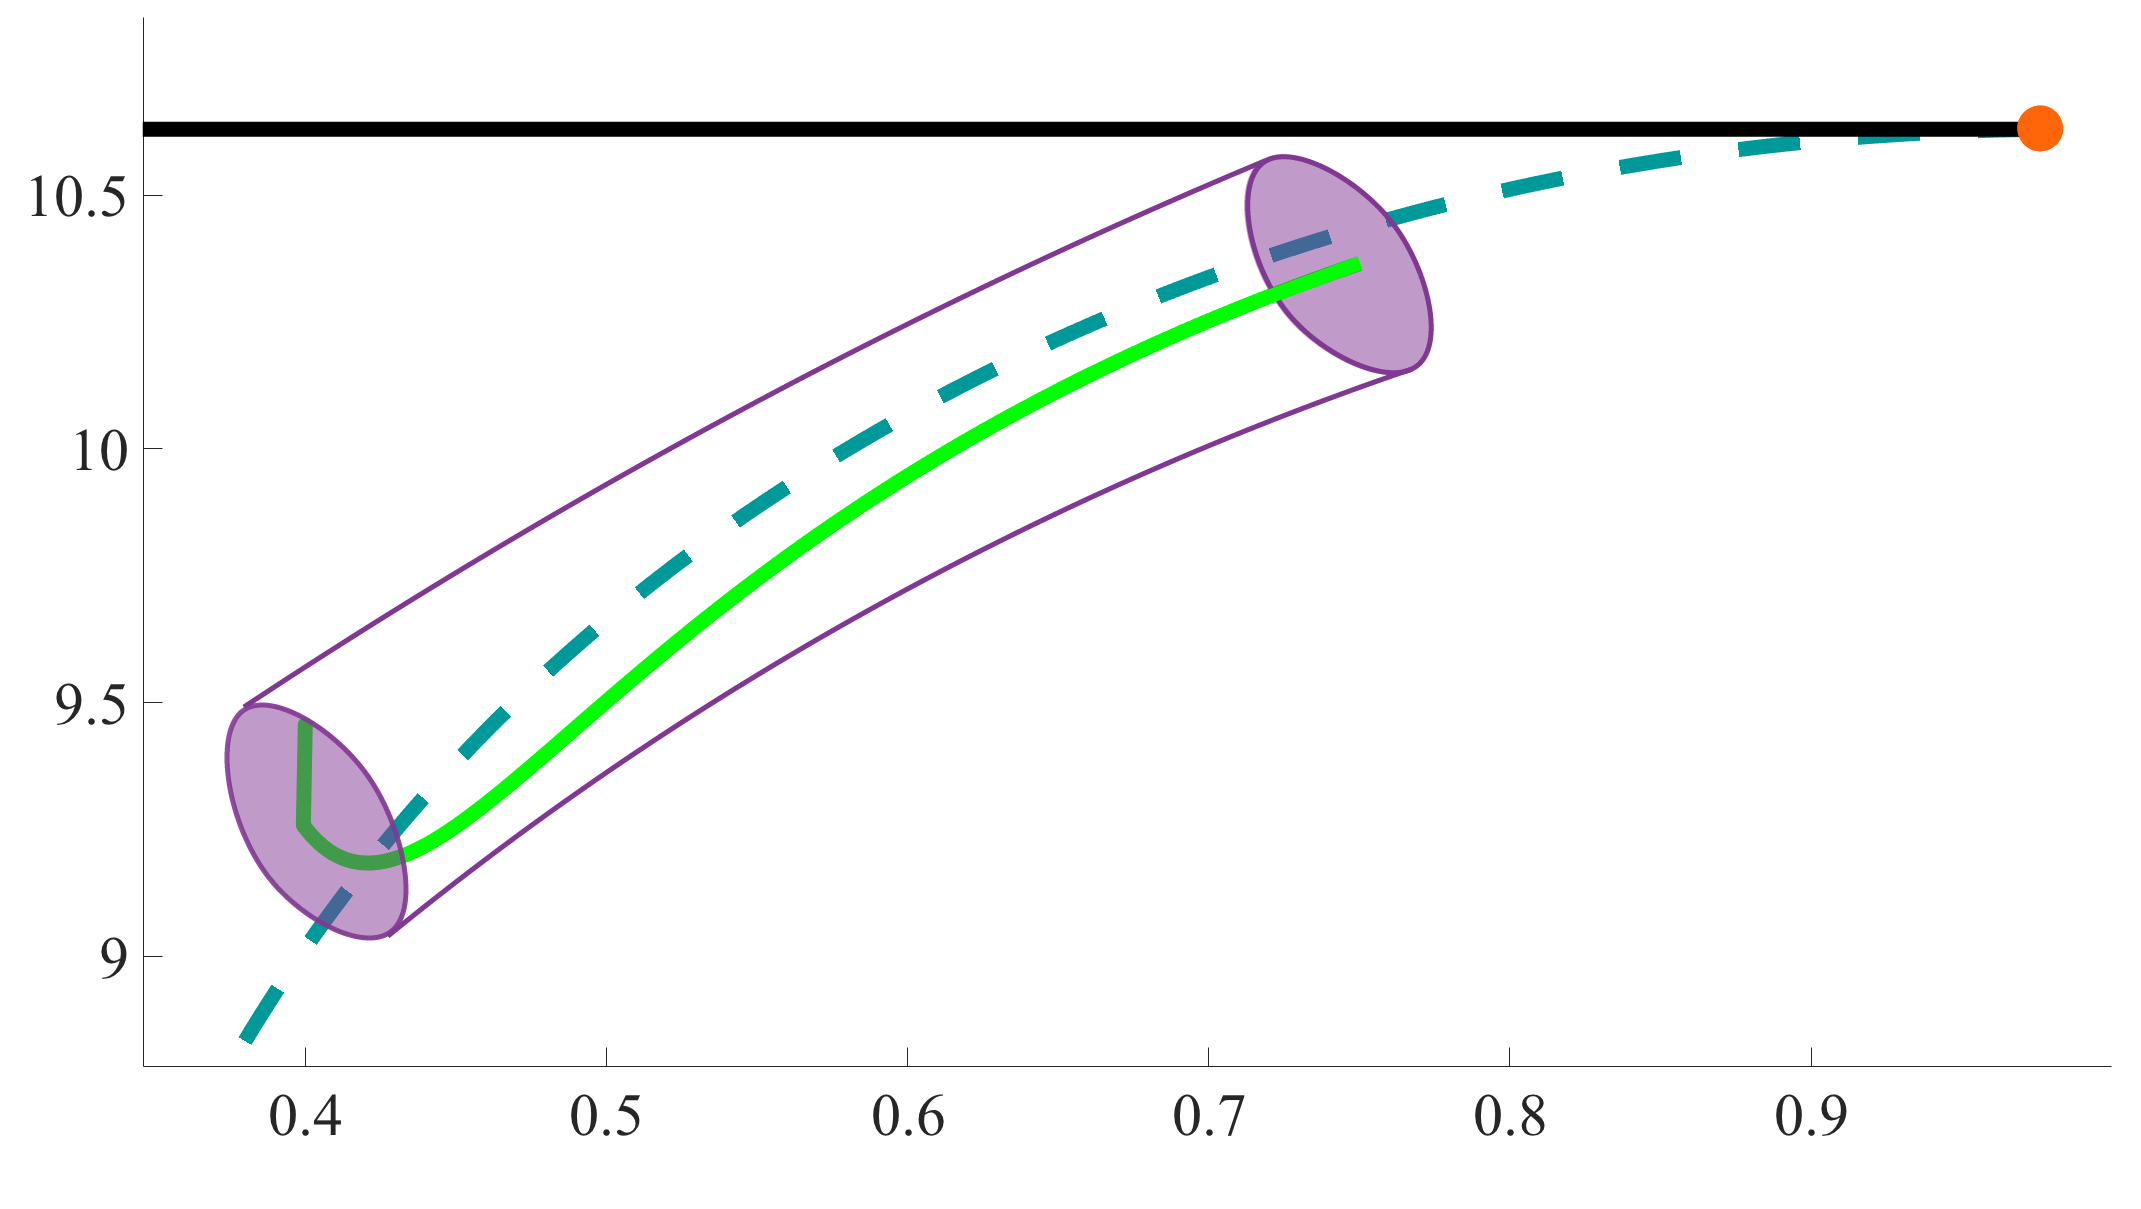
\includegraphics[width=11cm]{./figures_raw/paper_slow.eps}}
	    \put(196.5,153.5){$F_1$}
	    \put(173.5,148){$D_\delta(B_{\mathrm{out}})$}
	    \put(107,127){$D_\delta(B_{\mathrm{in}})$}
	    \put(121.5,110){$C^3$}
	    \put(120,151){$C^4_+$}
	    \put(147.5,135.25){$S^3$}
	    \put(148,139.25){$\uparrow$}
	    \put(97.5,156){$A$}
	    \put(95,143.5){\footnotesize $9.75$}
	    \put(95,114.25){\footnotesize $7.25$}
            \put(206,97){$B$}
            \put(120.75,98){\footnotesize$0.3$}
            \put(142.25,98){\footnotesize$0.5$}
            \put(163.8,98){\footnotesize$0.7$}
            \put(185.25,98){\footnotesize$0.9$}
	\end{picture}
	\caption{}
\end{figure}

\newpage


%%%%%%%%%%%%%%%%%%%%%%%%%%%%
%%% Figure 3: Stable manifold numerical set up %%%
%%%%%%%%%%%%%%%%%%%%%%%%%%%%

\begin{figure}
\begin{picture}(172.75,89)(2,-0.5)
\put(0,45){
	\begin{picture}(85,43)(5,7)
	\put(10.25,10){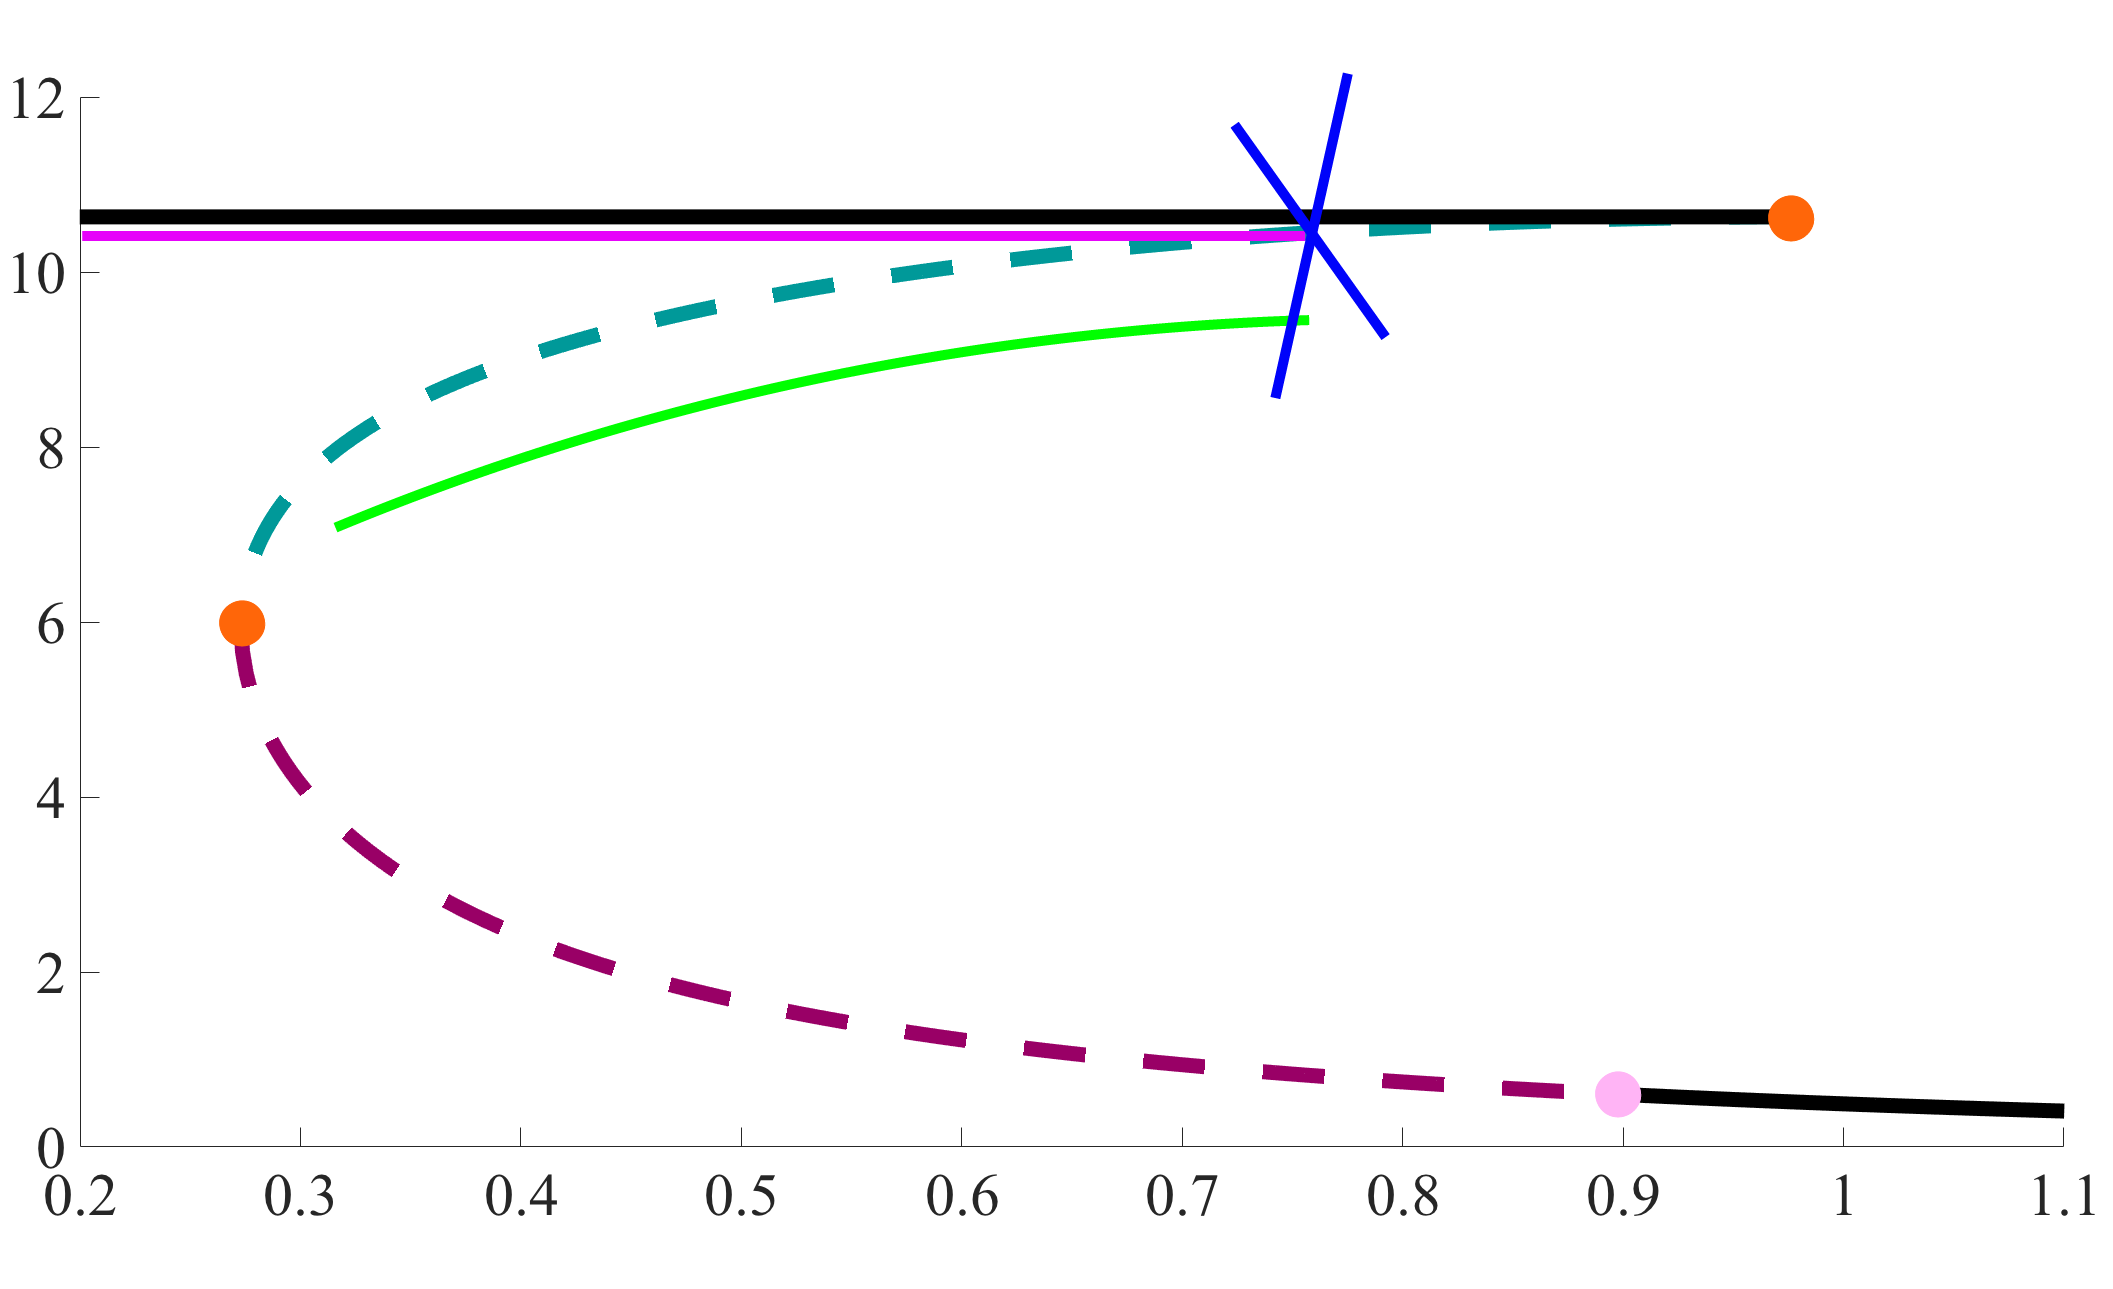
\includegraphics[width=8cm]{./figures_raw/step1.eps}}
        \put(72,37.75){$E^s(p_{\mathrm{out}})$}
        \put(20,40){$\widehat{\Sigma}$}
	\put(81,44){$F_1$}
        \put(19,29){$F_2$}
        \put(72.5,13.5){$H$}
        \put(80,13){$C^4_-$}
        \put(50,38){$S^3$}
        \put(50,15){$C^2$}
        \put(7,46){$A$}
        \put(6,39){\footnotesize $9.0$}
        \put(6,19){\footnotesize $3.0$}
	\put(24.5,7.5){\footnotesize $0.3$}
	\put(40.4,7.5){\footnotesize $0.5$}
	\put(56.4,7.5){\footnotesize $0.7$}
	\put(72.2,7.5){\footnotesize $0.9$}
	\put(86,6.9){$B$}
	\put(13,13.5){(a)}
	\put(25,20){$q$}
	\end{picture}
	\caption{}
	}

\put(88,45){
	\begin{picture}(85,43)(5,7)
	\put(10.25,10){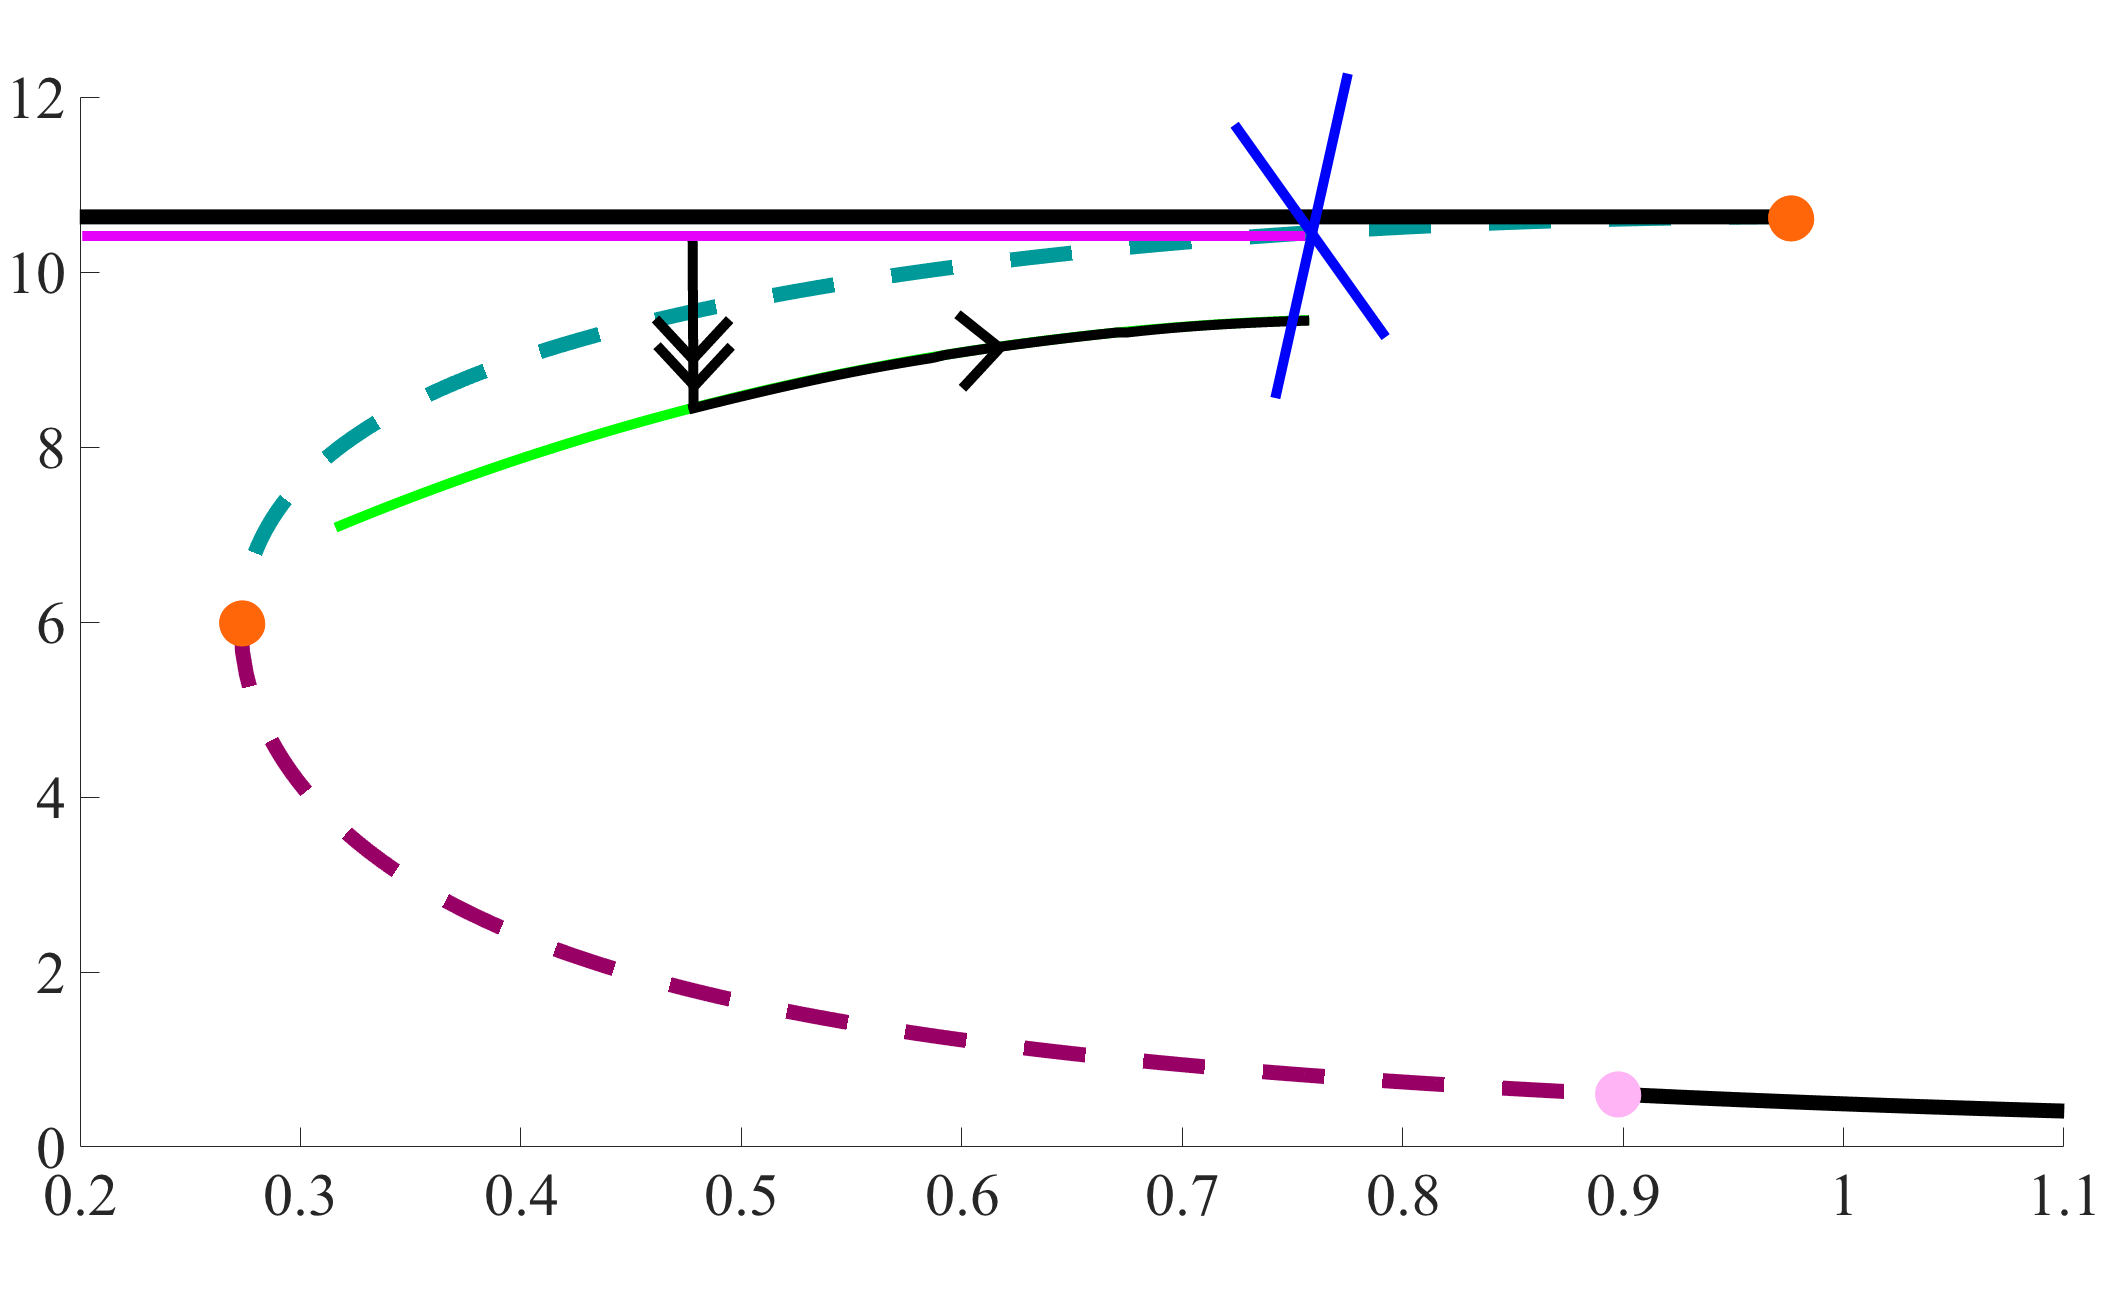
\includegraphics[width=8cm]{./figures_raw/step2.eps}}
        \put(72,37.75){$E^s(p_{\mathrm{out}})$}
        \put(18,40){$\widehat{\Sigma}$}
	\put(81,44){$F_1$}
        \put(19,29){$F_2$}
        \put(72.5,13.5){$H$}
        \put(80,13){$C^4_-$}
        \put(7,46){$A$}
        \put(50,15){$C^2$}
        \put(55,39.25){$\mathbf{u}$}
        \put(6,39){\footnotesize $9.0$}
        \put(6,19){\footnotesize $3.0$}
	\put(24.5,7.5){\footnotesize $0.3$}
	\put(40.4,7.5){\footnotesize $0.5$}
	\put(56.4,7.5){\footnotesize $0.7$}
	\put(72.2,7.5){\footnotesize $0.9$}
	\put(86,6.9){$B$}
	\put(13,13.5){(b)}
	\put(25,20){$q$}
	\end{picture}
	\caption{}
	}
	
\put(0,0){
	\begin{picture}(85,43)(5,7)
	\put(10.25,10){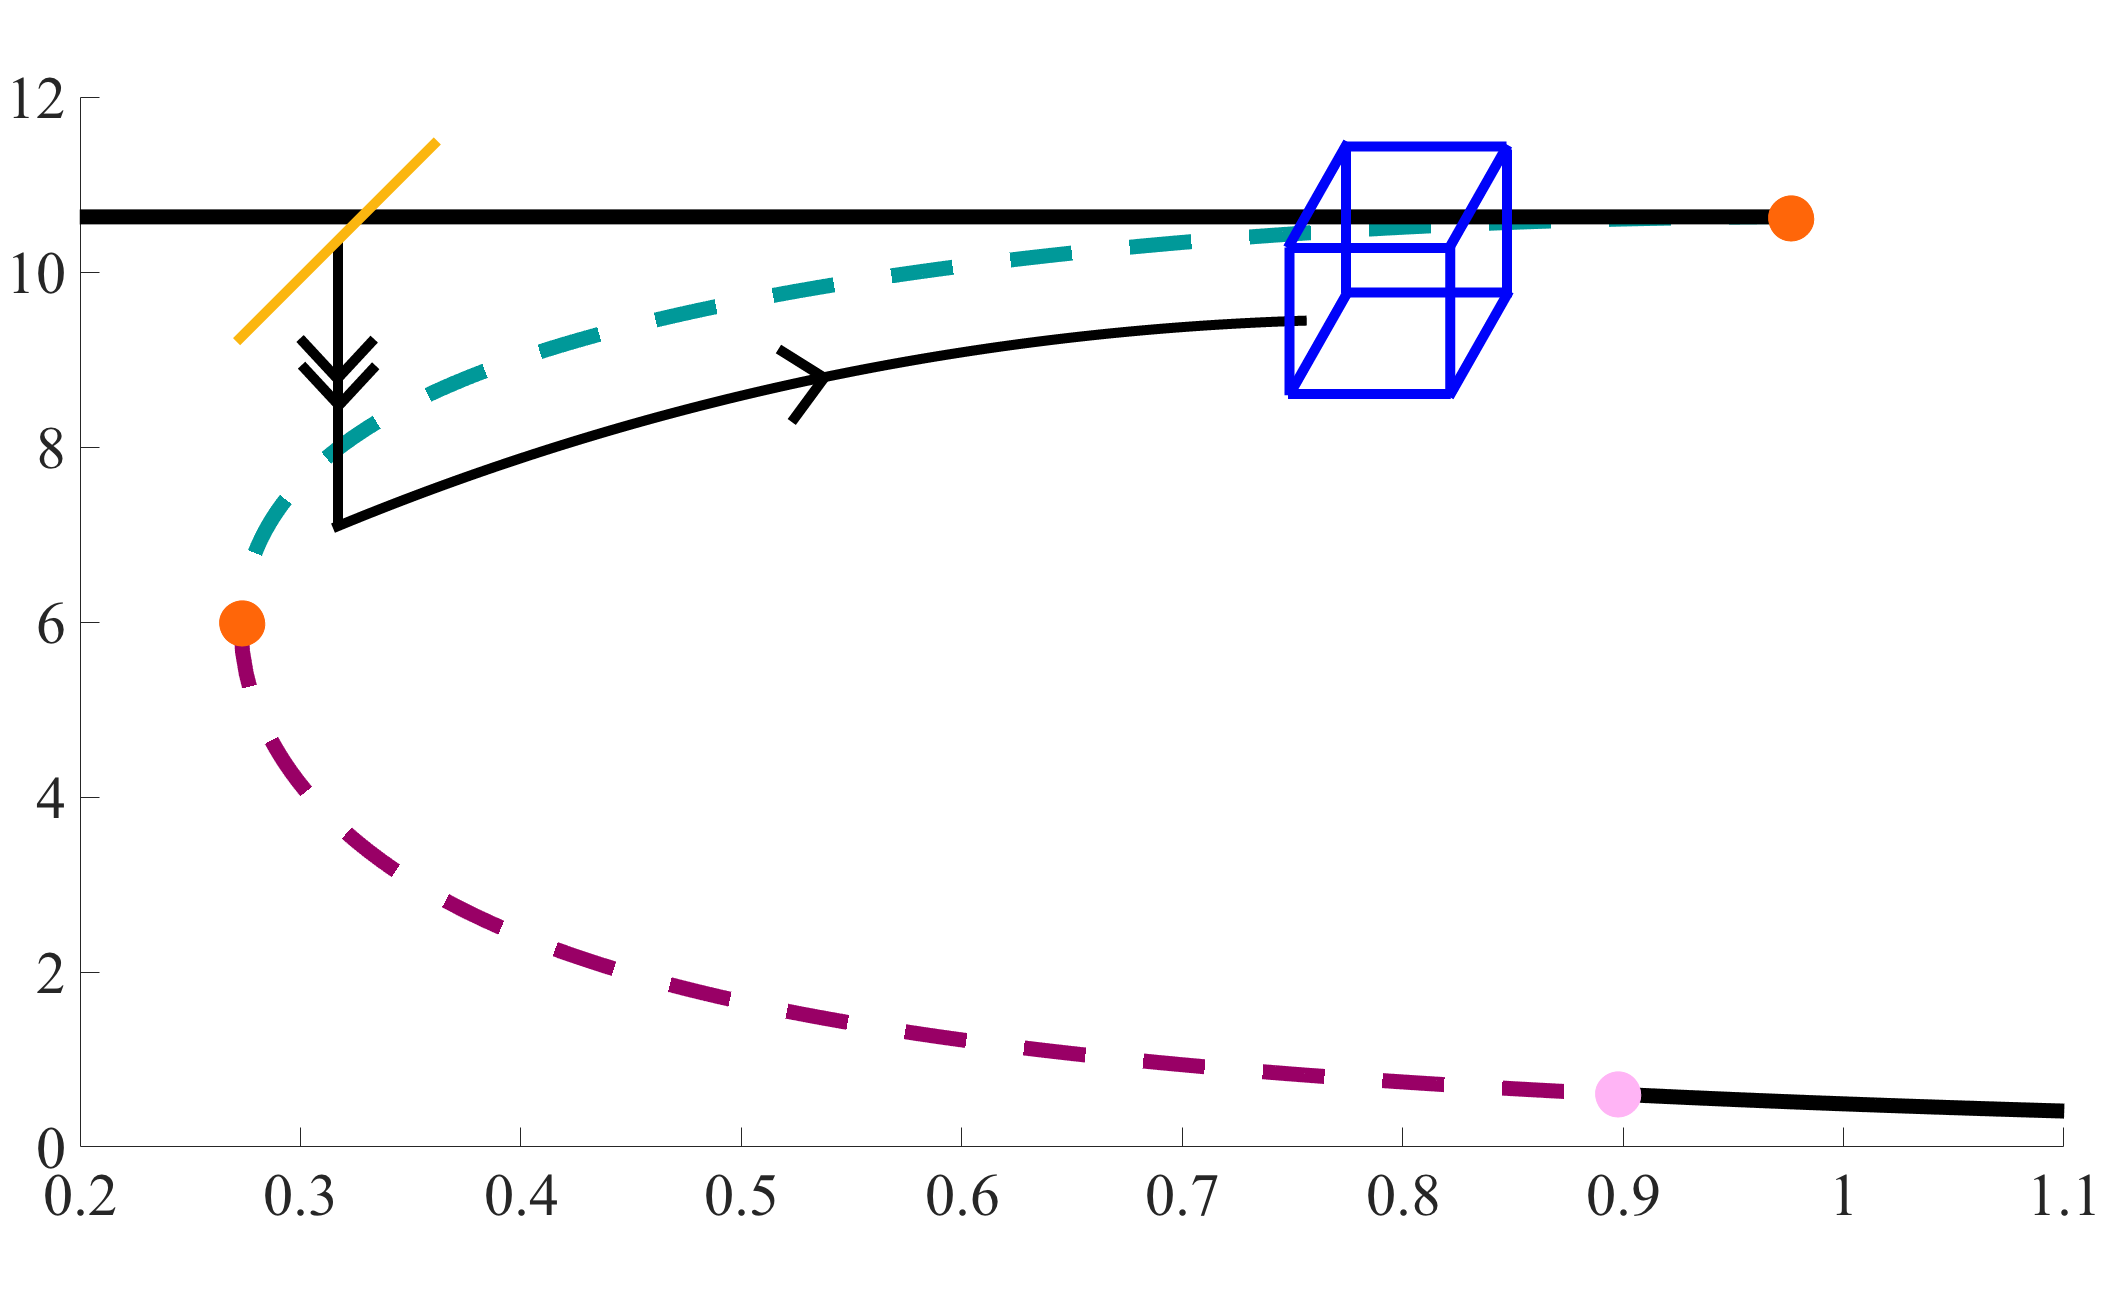
\includegraphics[width=8cm]{./figures_raw/step3.eps}}
 	\put(72,36.5){$\Omega$}
        \put(19,40){$\psi$}
	\put(81,44){$F_1$}
        \put(19,29){$F_2$}
        \put(72.5,13.5){$H$}
        \put(7,46){$A$}
        \put(80,13){$C^4_-$}
        \put(50,15){$C^2$}
        \put(50,38.5){$\mathbf{u}$}        
        \put(6,39){\footnotesize $9.0$}
        \put(6,19){\footnotesize $3.0$}
	\put(24.5,7.5){\footnotesize $0.3$}
	\put(40.4,7.5){\footnotesize $0.5$}
	\put(56.4,7.5){\footnotesize $0.7$}
	\put(72.2,7.5){\footnotesize $0.9$}
	\put(86,6.9){$B$}
	\put(13,13.5){(c)}
	\put(25,20){$q$}
	\end{picture}
	}
\put(89,0){\begin{picture}(85,43)(5,7)
	\put(10.25,10){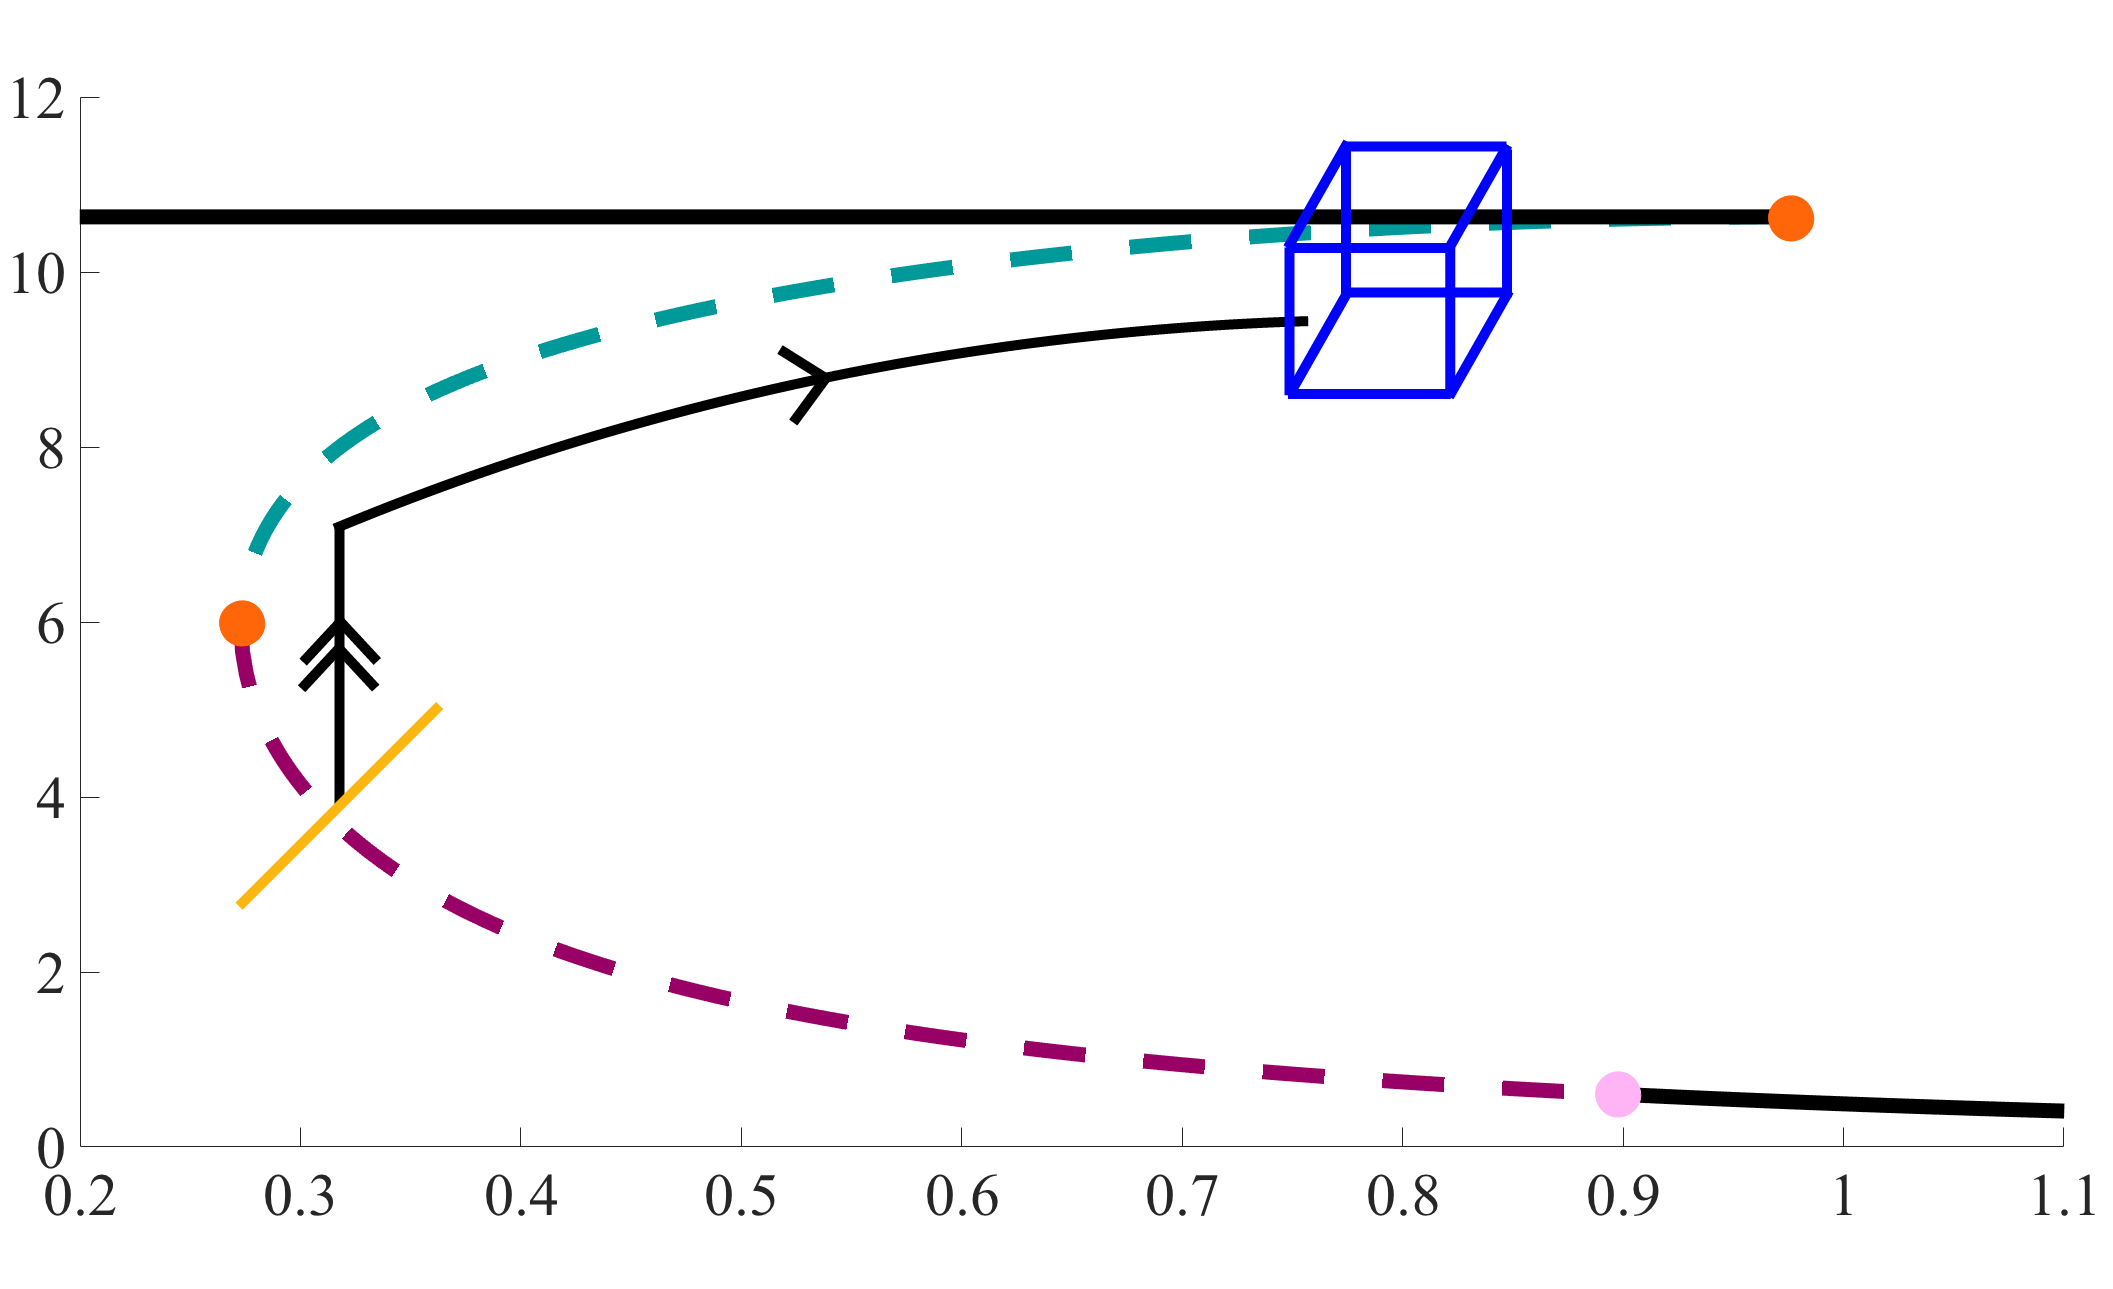
\includegraphics[width=8cm]{./figures_raw/step4.eps}}
	\put(72,36.5){$\Omega$}
        \put(33,20){$\psi$}
	\put(81,44){$F_1$}
        \put(19,29){$F_2$}
        \put(72.5,13.5){$H$}
        \put(7,46){$A$}
        \put(50,15){$C^2$}
        \put(80,13){$C^4_-$}   
        \put(20,41.5){$C^4_+$}
        \put(50,38.5){$\mathbf{u}$}        
        \put(6,39){\footnotesize $9.0$}
        \put(6,19){\footnotesize $3.0$}
	\put(24.5,7.5){\footnotesize $0.3$}
	\put(40.4,7.5){\footnotesize $0.5$}
	\put(56.4,7.5){\footnotesize $0.7$}
	\put(72.2,7.5){\footnotesize $0.9$}
	\put(86,6.9){$B$}
	\put(13,13.5){(d)}
	\put(25,20){$q$}
	\end{picture}
	\caption{}
}
\end{picture}
\end{figure}

\newpage

%%%%%%%%%%%%%%%%%%%%%%%%%%%
%%% Figure 4: One piece of the stable manifold %%%
%%%%%%%%%%%%%%%%%%%%%%%%%%%

\begin{figure}
\begin{picture}(134,179)(47.5,59.5)
\put(50,140){
	\begin{picture}(180,100)(0,0)
	    \put(0,0){\includegraphics[width=12.6cm]{./figures_raw/one_piece_paper_BAX.png}}
	    \put(115,65){$W^{s}_{\widehat{\Sigma}}$}
	    \put(120,24){$\widehat{\Sigma}$}
	    \put(-0.75,6){$\Omega$}
	    \put(101,94){$C^3$}
	    \put(70,3){$C^{4}_{+}$}
	    \put(13,81){(a)}
	\end{picture}
	\caption{}
}

\put(50,58){
	\begin{picture}(180,100)(0,0)
	    \put(0,0){\includegraphics[width=12.6cm]{./figures_raw/one_piece_paper_BAY.png}}
	    \put(123.5,46){$W^{s}_{\widehat{\Sigma}}$}
	    \put(-3,5.5){$\Omega$}
	    \put(108,79.5){$C^3$}
	    \put(70,3){$C^{4}_{+}$}
	    \put(123,4.5){$\widehat{\Sigma}$}
	    \put(13,60){(b)}
	\end{picture}
	\caption{}
}
\end{picture}
\end{figure}


\newpage



%%%%%%%%%%%%%%%%%%%%%%%%%%%%
%%% Figure 5: Two pieces of the stable manifold %%%
%%%%%%%%%%%%%%%%%%%%%%%%%%%%

\begin{figure}
\begin{picture}(121,170.5)(57,62.5)
\put(50,140){
	\begin{picture}(180,100)(0,0)
	    \put(0,0){\includegraphics[width=12.6cm]{./figures_raw/two_pieces_paper_BAX.eps}}
	    \put(110,50.5){$W^{s}_{\widehat{\Sigma}}$}
	    \put(122,32){$\widehat{\Sigma}$}
	    \put(13,62){$\Sigma_1$}
	    \put(47.5,5){$\Omega$}
	    \put(30,83){$C^2$}
	    \put(99,56){$C^3$}
	    \put(94,64){$F_2$}
	    \put(88,9){$C^{4}_{+}$}
	    \put(13,89.5){(a)}
	\end{picture}
	\caption{}
}

\put(50,60){
	\begin{picture}(180,100)(0,0)
	    \put(0,2){\includegraphics[width=12.6cm]{./figures_raw/two_pieces_paper_BAY.eps}}
	    \put(110,39.5){$W^{s}_{\widehat{\Sigma}}$}
	    \put(13,27){$\Sigma_1$}
	    \put(47.25,7){$\Omega$}
	    \put(82.5,60){$C^2$}
	    \put(92,45){$C^3$}
	    \put(88,12){$C^{4}_{+}$}
	    \put(123.5,22.5){$\widehat{\Sigma}$}
	    \put(94.5,54){$F_2$}
	    \put(13,60){(b)}
	\end{picture}
	\caption{}
}
\end{picture}
\end{figure}


\newpage


%%%%%%%%%%%%%%%%%%%%%%%%%%%%
%%% Figure 6: Five pieces of the stable manifold %%%
%%%%%%%%%%%%%%%%%%%%%%%%%%%%

\begin{figure}
\begin{picture}(120,196)(58,36.5)
\put(50,140){
	\begin{picture}(180,100)(0,0)
	    \put(0,0){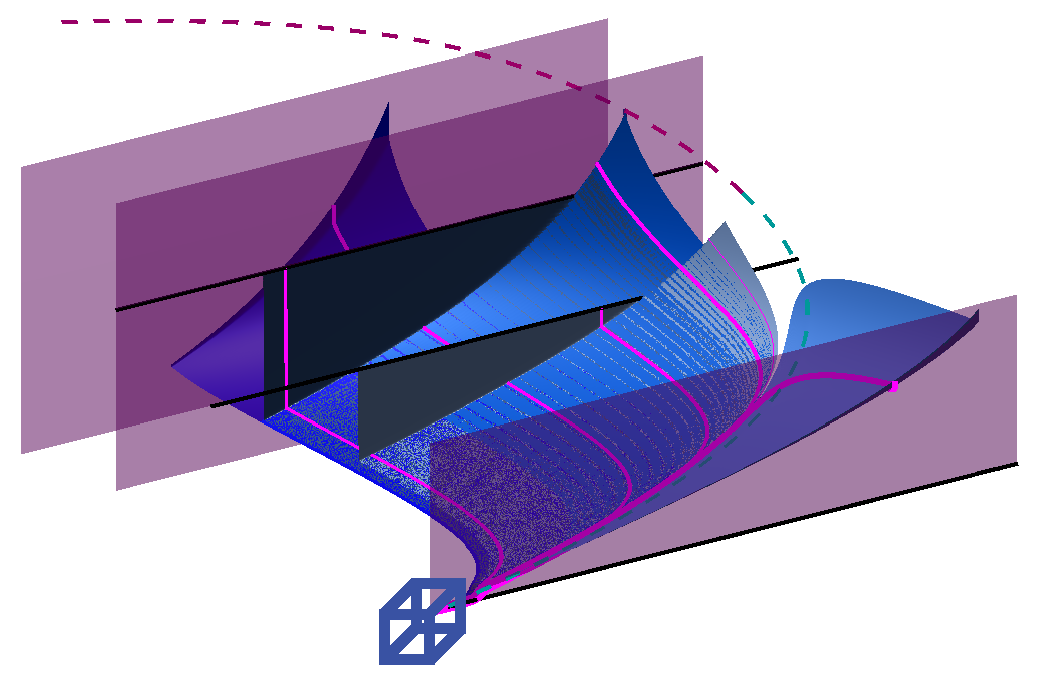
\includegraphics[width=12.6cm]{./figures_raw/five_pieces_paper_BAX.eps}}
	    \put(110,51){$W^{s}_{\widehat{\Sigma}}$}
	    \put(122,35){$\widehat{\Sigma}$}
	    \put(13,62){$\Sigma_1$}
	    \put(22,57){$\Sigma_2$}
	    \put(24,46.5){$\Sigma_3$}
	    \put(27,30){$\Sigma_4$}
	    \put(48.25,5){$\Omega$}
	    \put(94,64){$F_2$}
	    \put(30,83){$C^2$}
	    \put(99,56){$C^3$}
	    \put(88,9.75){$C^{4}_{+}$}
	    \put(13,89.5){(a)}
	\end{picture}
	\caption{}
}

\put(50,35){
	\begin{picture}(180,100)(0,0)
	    \put(0,0){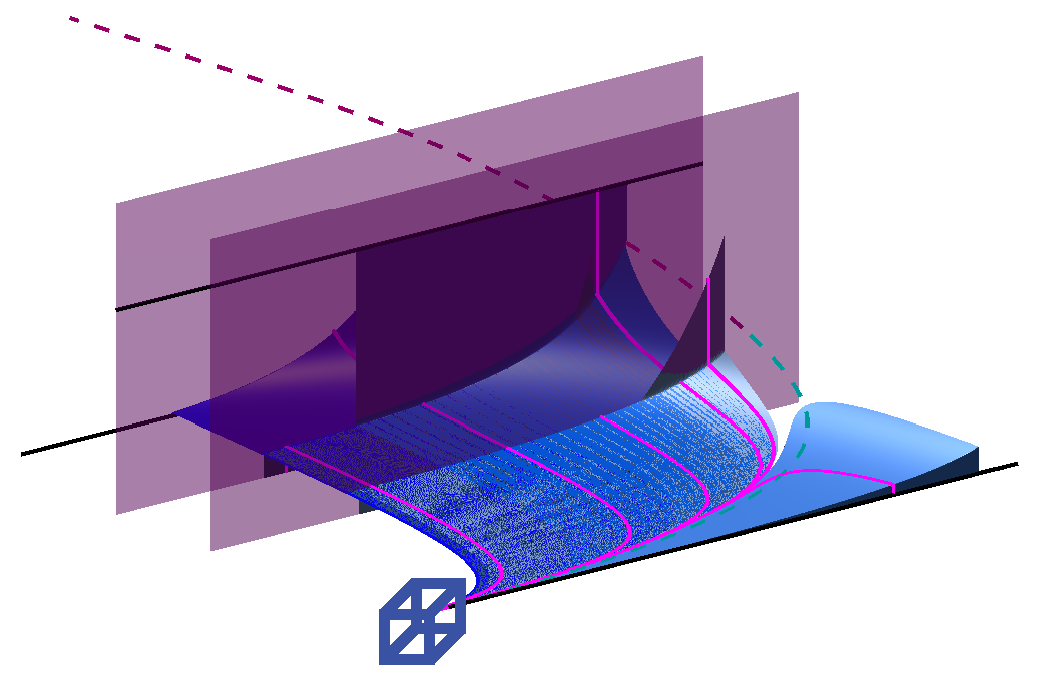
\includegraphics[width=12.6cm]{./figures_raw/five_pieces_paper_BAY.eps}}
	    \put(110,38.5){$W^{s}_{\widehat{\Sigma}}$}
	    \put(13,26){$\Sigma_1$}
	    \put(23,72){$\Sigma_2$}
	    \put(22,53){$\Sigma_3$}
	    \put(33,65){$\Sigma_4$}
	    \put(48,6){$\Omega$}
	    \put(56.5,90){$C^2$}
	    \put(98.5,45){$C^3$}
	    \put(88,11.5){$C^{4}_{+}$}
	    \put(94.5,54){$F_2$}
	    \put(122,21){$\widehat{\Sigma}$}
	    \put(13,81){(b)}
	\end{picture}
	\caption{}
}
\end{picture}
\end{figure}
\newpage


%%%%%%%%%%%%%%%%%%%%%%%%%%%
%%% Figure 7: One piece of the unstable manifold %%
%%%%%%%%%%%%%%%%%%%%%%%%%%%
\begin{figure}
\begin{picture}(131,142.5)(99.5,104.5)
\put(100,160){
	\begin{picture}(180,100)(0,0)
	    \put(0,24){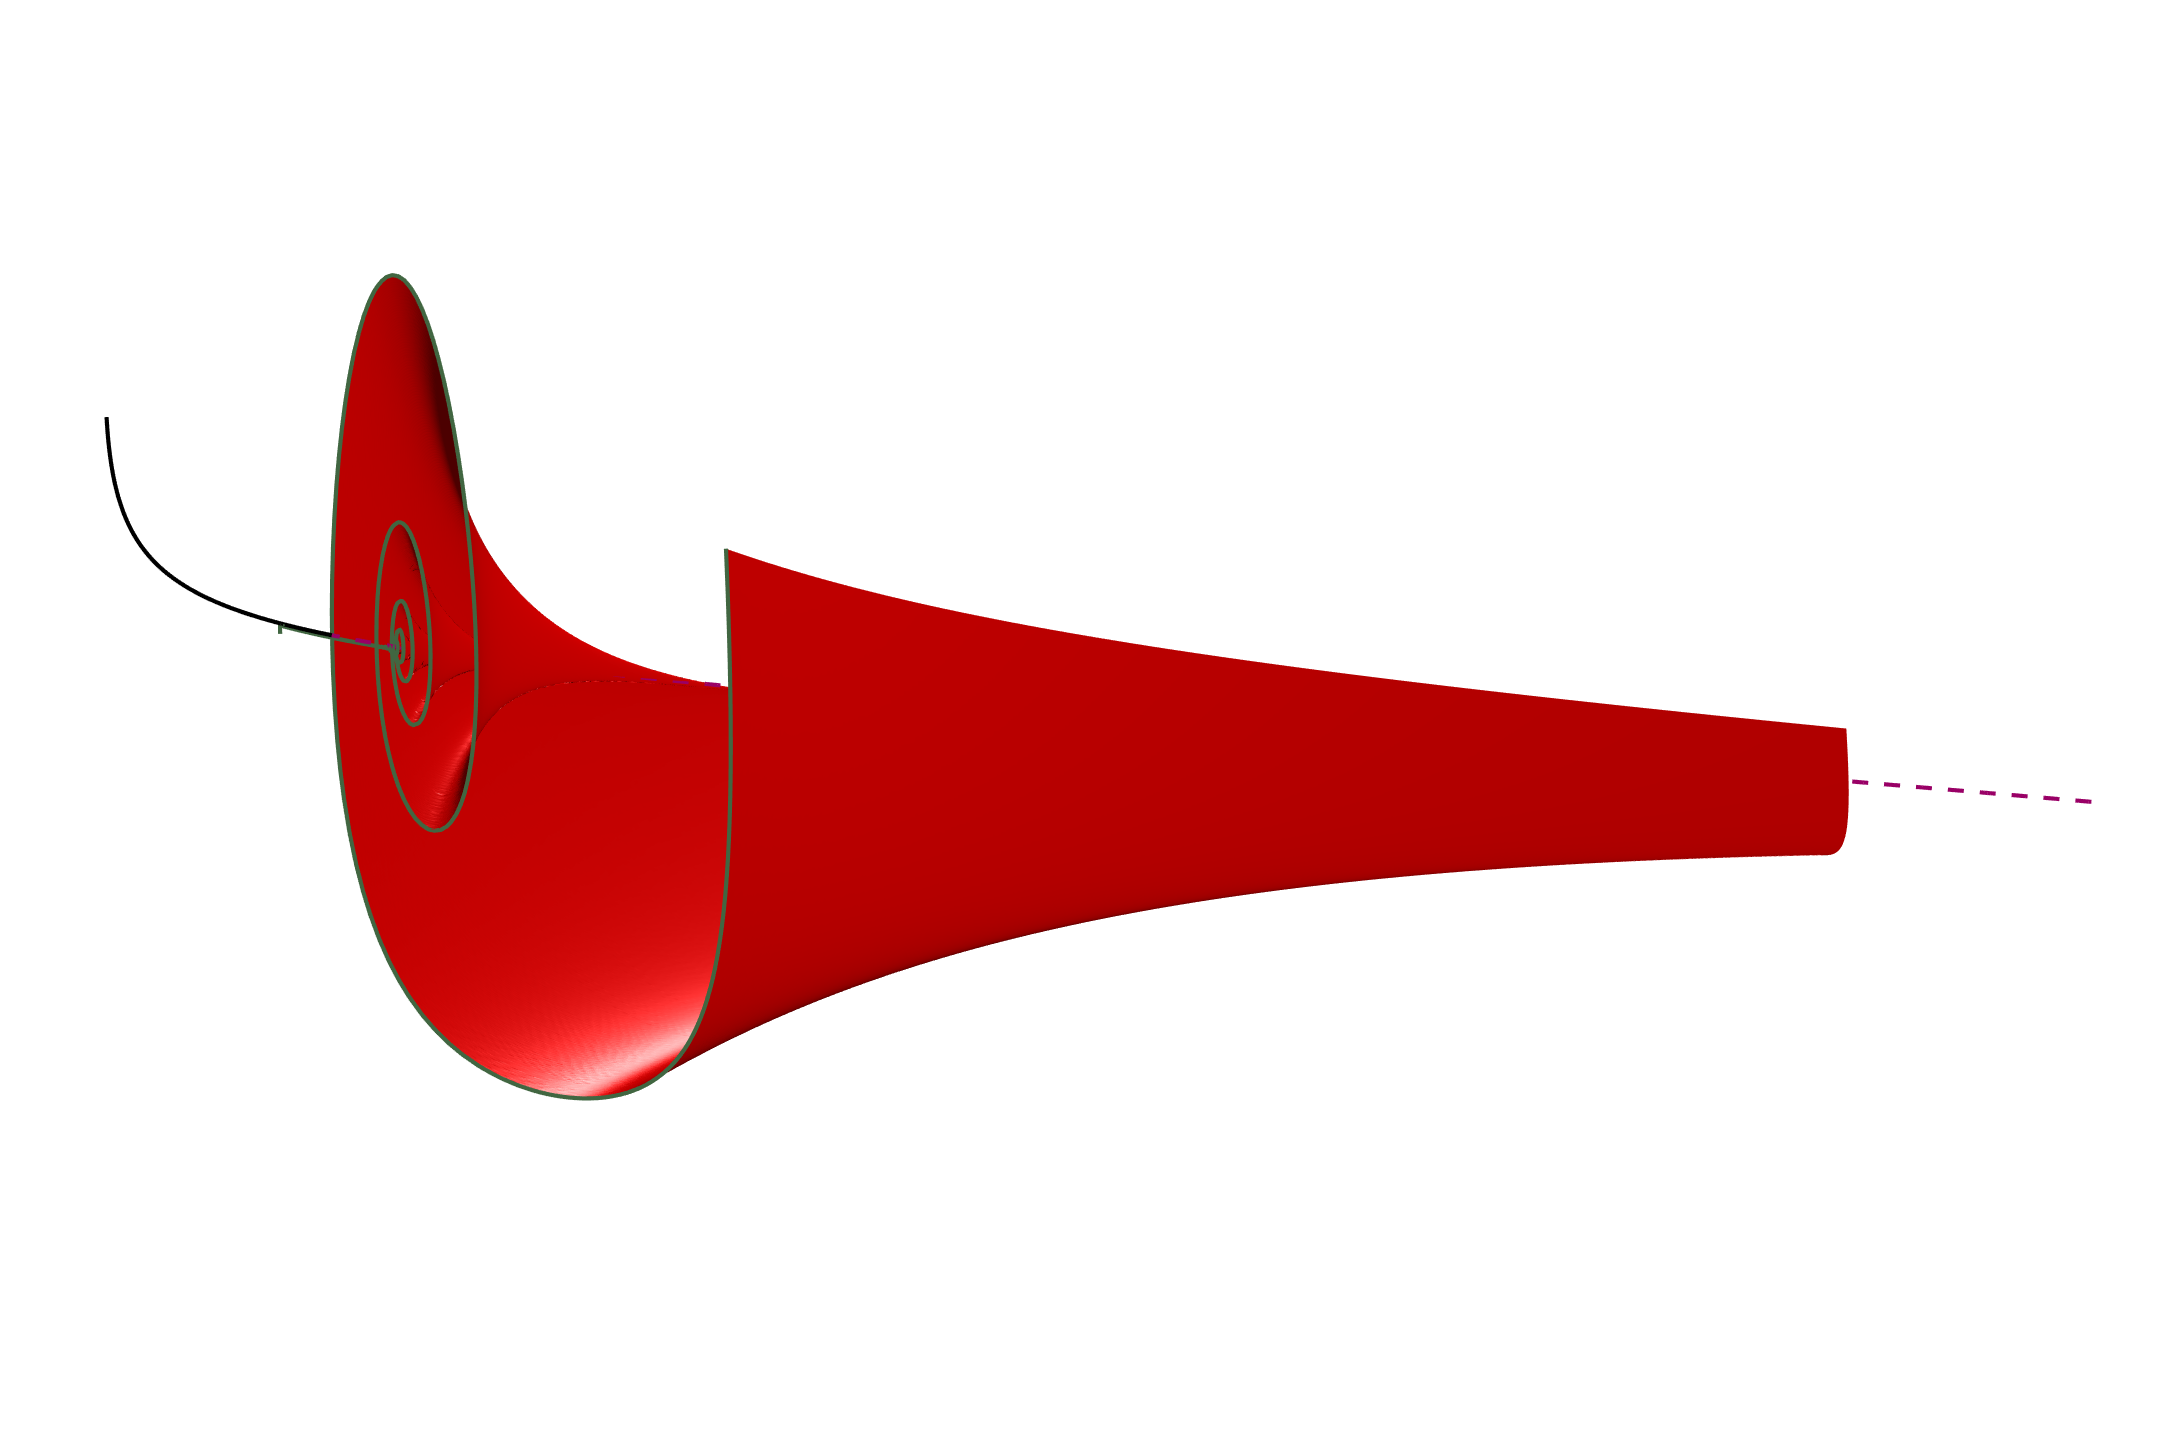
\includegraphics[width=12.6cm]{./figures_raw/unstable_piece_BAX.eps}}
	    \put(70,59.5){$W^{u}_{r^*}\cap\mathscr{R}$}
	    \put(70,36){$W^{u}_{r^*}$}
	    \put(11,70){$\Phi$}
	     \put(15,55){$H$}
	    \put(0,70){$C^4_-$}
	    \put(118,49){$C^2$}
	    \put(2,81){(a)}
	\end{picture}
	\caption{}
}

\put(100,85){
	\begin{picture}(180,100)(0,0)
	    \put(3,19.5){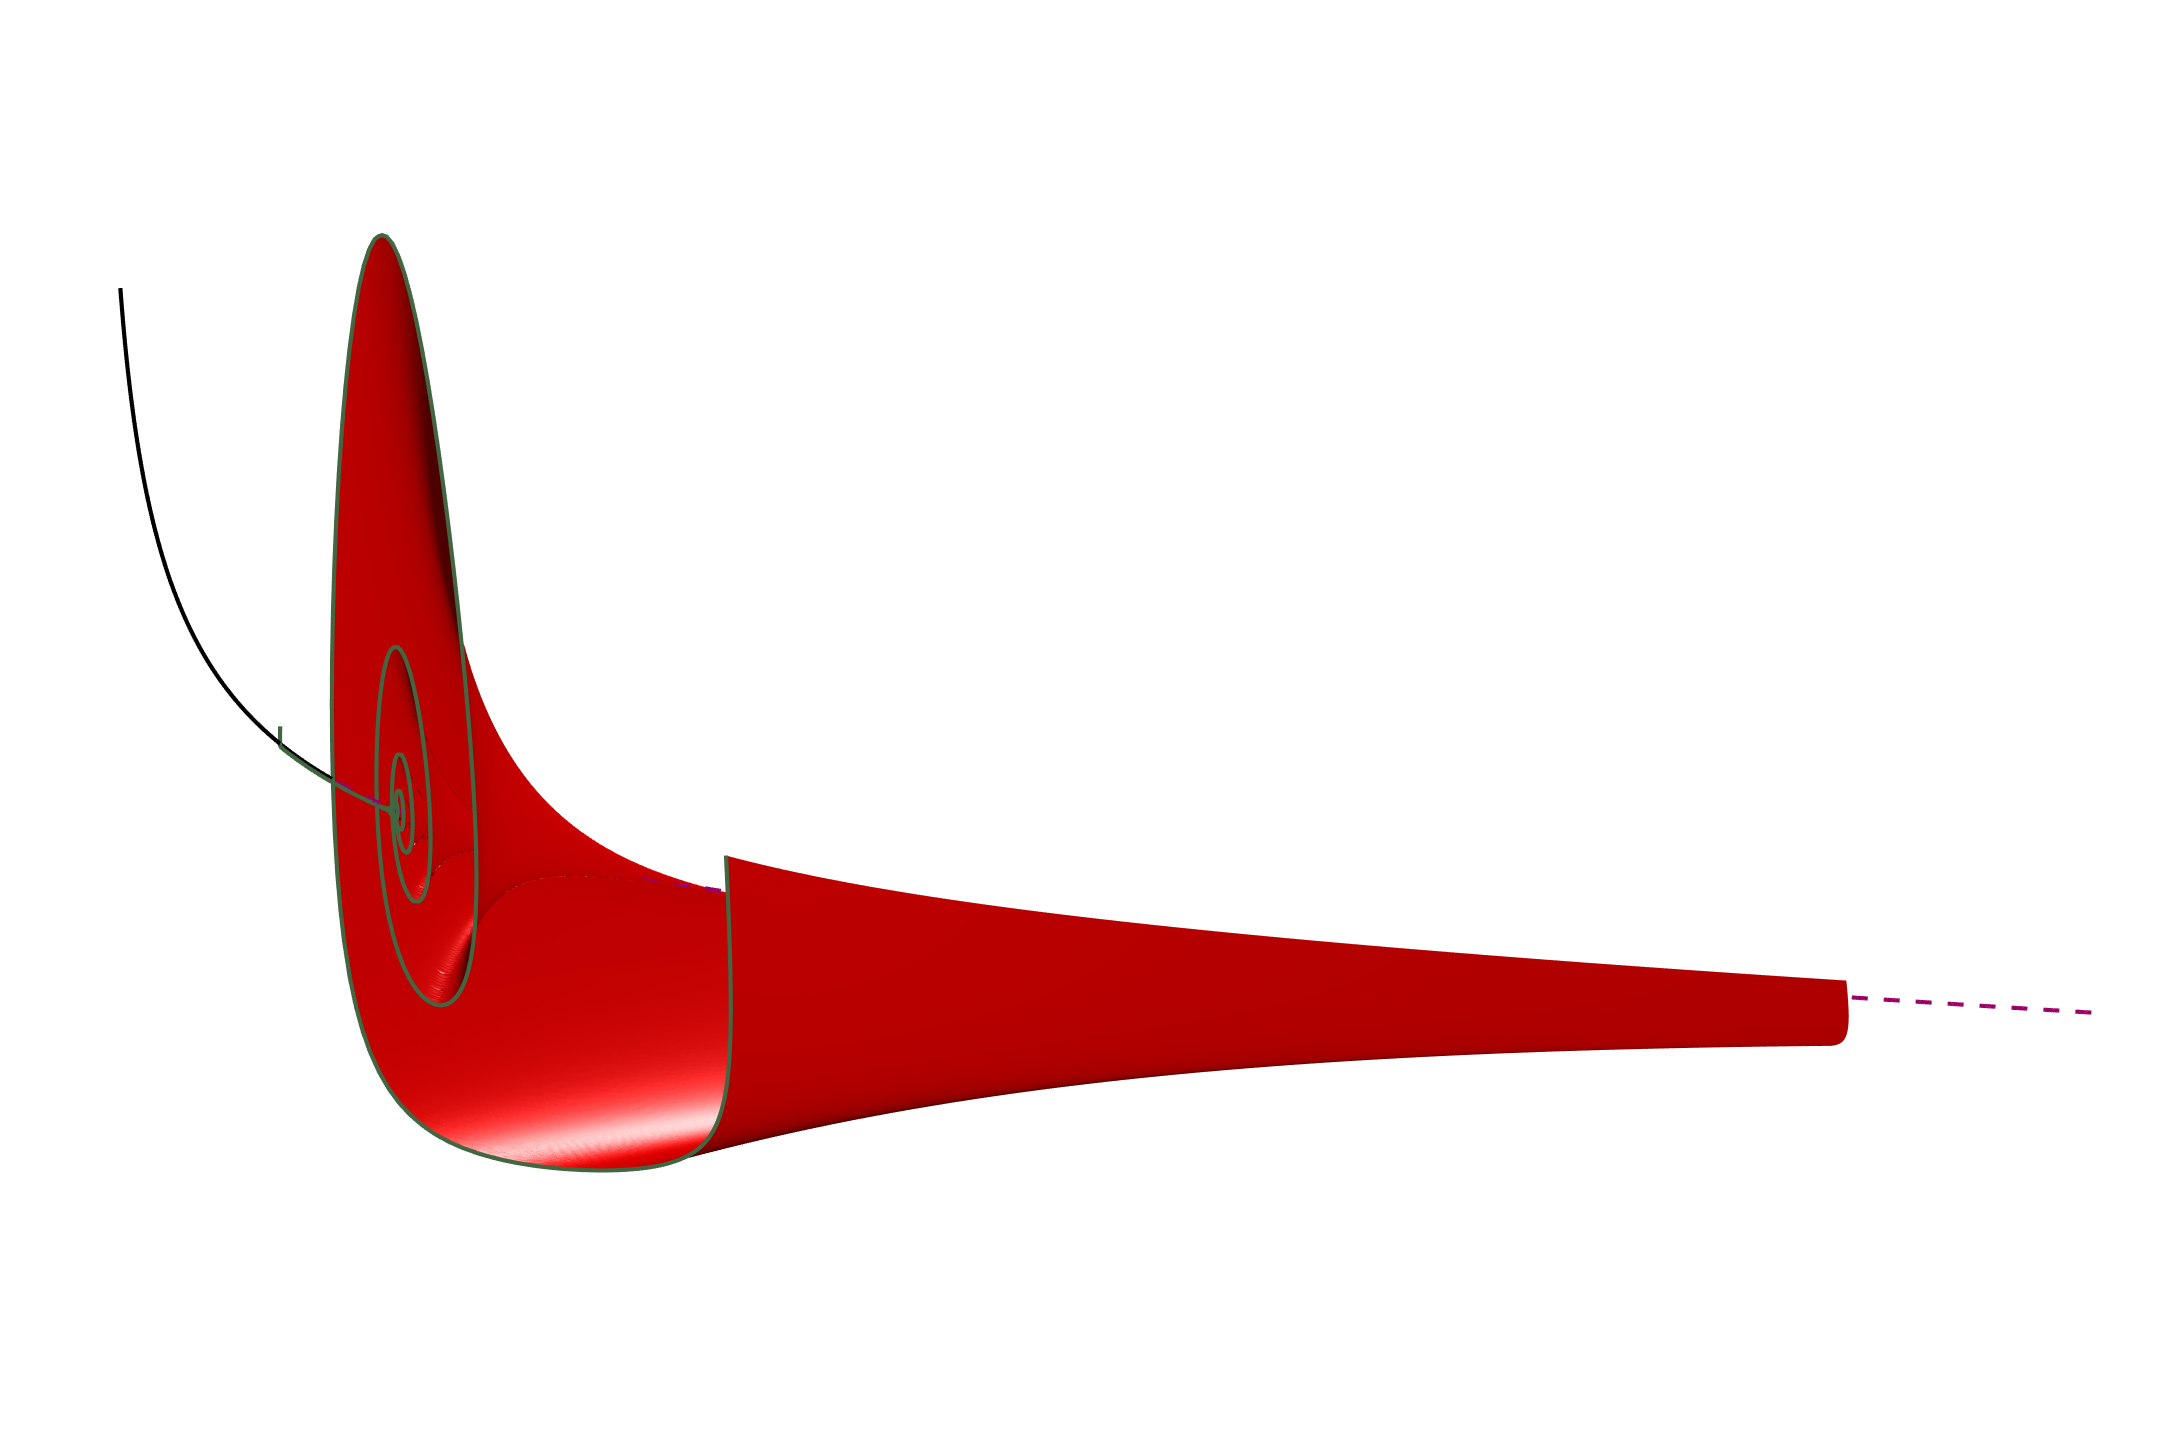
\includegraphics[width=12.6cm]{./figures_raw/unstable_piece_BAY.eps}}
	    \put(70,40){$W^{u}_{r^*}\cap\mathscr{R}$}
	    \put(70,23.5){$W^{u}_{r^*}$}
	    \put(14,62.5){$\Phi$}
	    \put(18,45){$H$}
	    \put(4.5,73){$C^4_-$}
	    \put(118,34){$C^2$}
	    \put(2,87){(b)}
	\end{picture}
	\caption{}
}
\end{picture}
\end{figure}



%%%%%%%%%%%%%%%%%%%%%%%%%%
%%% Figure 8: Lin's method numerical set up %%%
%%%%%%%%%%%%%%%%%%%%%%%%%%

\begin{figure}
\begin{picture}(173,89)(2,-0.5)
\put(0,45){
	\begin{picture}(85,43)(5,7)
	\put(10.25,10){\includegraphics[width=8cm]{./figures_raw/Lin1.eps}}
        \put(50,38){$S^3$}
        \put(50,17){$S^2$}
        \put(7,46){$A$}
        \put(6,39){\footnotesize $9.0$}
        \put(6,19){\footnotesize $3.0$}
	\put(24.5,7.5){\footnotesize $0.3$}
	\put(40.4,7.5){\footnotesize $0.5$}
	\put(56.4,7.5){\footnotesize $0.7$}
	\put(72.2,7.5){\footnotesize $0.9$}
	\put(86,6.9){$B$}
	\put(25,20){$q$}
	\put(81,44){$F_1$}
        \put(73,13.5){$H$}
        	\put(80,13){$C^4_-$}
        \put(20,41.5){$C^4_+$}
	\put(13,13.5){(a)}
	\end{picture}
	\caption{}
	}

\put(88,42){
	\begin{picture}(85,43)(5,7)
	\put(10.25,10){\includegraphics[width=8cm]{./figures_raw/Lin2.eps}}
        \put(49.5,41.5){$\mathbf{u}$}
        \put(7,49){$A$}
        \put(6,42){\footnotesize $9.0$}
        \put(6,22){\footnotesize $3.0$}
	\put(24.5,10.5){\footnotesize $0.3$}
	\put(40.4,10.5){\footnotesize $0.5$}
	\put(56.4,10.5){\footnotesize $0.7$}
	\put(72.2,10.5){\footnotesize $0.9$}
	\put(86,10.1){$B$}
	\put(72,40.75){$E^s(p_{\mathrm{out}})$}
	\put(25,23){$q$}
	\put(80,16){$C^4_-$}
        \put(20,44.5){$C^4_+$}
        \put(50,18){$C^2$}
        	\put(81,47){$F_1$}
        \put(73,16.5){$H$}
	\put(13,16){(b)}
	\end{picture}
	\caption{}
	}
	
\put(0,0){
	\begin{picture}(85,43)(5,7)
	\put(10.25,10){\includegraphics[width=8cm]{./figures_raw/Lin3.eps}}
        \put(7,46){$A$}
        \put(49.25,38.5){$\mathbf{u}$}
        \put(62,16){$\mathbf{w}$}
        \put(35,26.5){$\eta/Z$}
        \put(6,39){\footnotesize $9.0$}
        \put(6,19){\footnotesize $3.0$}
	\put(24.5,7.5){\footnotesize $0.3$}
	\put(40.4,7.5){\footnotesize $0.5$}
	\put(56.4,7.5){\footnotesize $0.7$}
	\put(72.2,7.5){\footnotesize $0.9$}
	\put(86,6.9){$B$}
	\put(72,37.75){$E^s(p_{\mathrm{out}})$}
	\put(72,17){$E^u(p_{\mathrm{in}})$}
	\put(20,41.5){$C^4_+$}
	\put(25,20){$q$}
	\put(13,13.5){(c)}
	\end{picture}
	}
\put(89,0){\begin{picture}(85,43)(5,7)
	\put(10.25,10){\includegraphics[width=8cm]{./figures_raw/Lin4.eps}}
	\put(61.25,40){$\mathbf{u}$}
        \put(62,16){$\mathbf{w}$}
        \put(7,46){$A$}
        \put(6,39){\footnotesize $9.0$}
        \put(6,19){\footnotesize $3.0$}
	\put(24.5,7.5){\footnotesize $0.3$}
	\put(40.4,7.5){\footnotesize $0.5$}
	\put(56.4,7.5){\footnotesize $0.7$}
	\put(72.2,7.5){\footnotesize $0.9$}
	\put(86,6.9){$B$}
	\put(72,37.75){$E^s(p_{\mathrm{out}})$}
	\put(72,17){$E^u(p_{\mathrm{in}})$}
	\put(20,41.5){$C^4_+$}
	\put(25,20){$q$}
	\put(13,13.5){(d)}
	\end{picture}
	\caption{}
}
\end{picture}
\end{figure}

\newpage



%%%%%%%%%%%%%%%%%%%%%%%%%%%%
%% Figure 9: Heteroclinic surface, numerical set up %%
%%%%%%%%%%%%%%%%%%%%%%%%%%%%

\begin{figure}
\begin{picture}(122,173)(52,48.5)
\put(50,140){
	\begin{picture}(180,100)(0,0)
	    \put(0,0){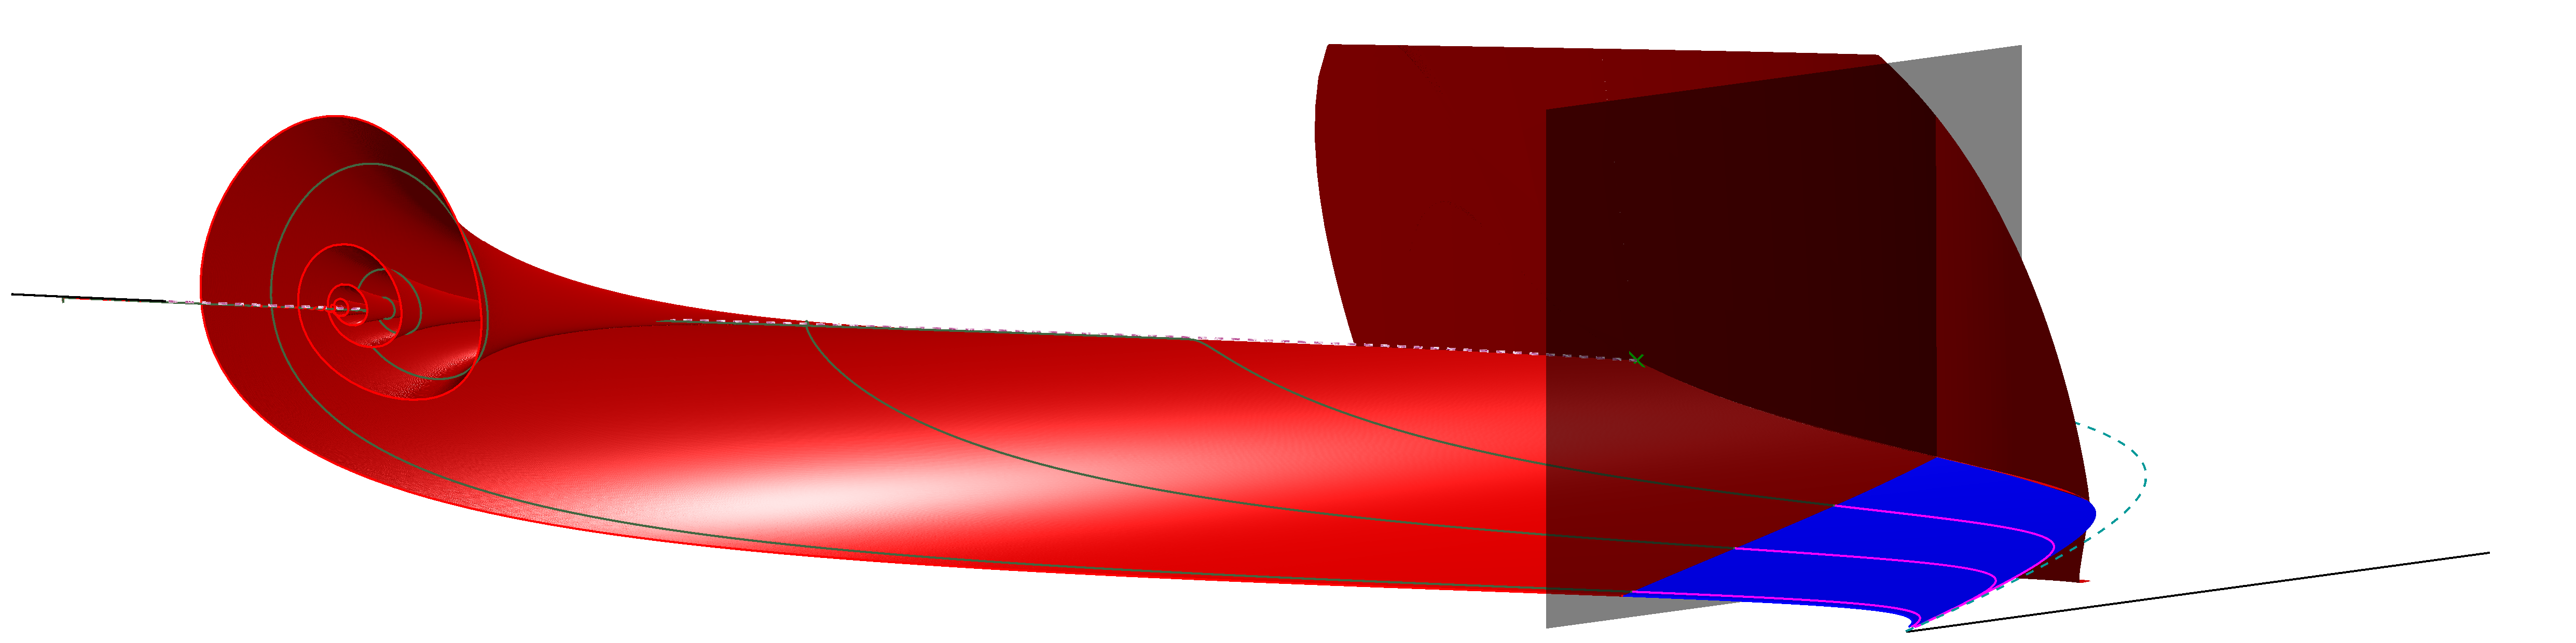
\includegraphics[width=12.6cm]{./figures_raw/hetclin_6_BAX.eps}}
	    \put(92.5,34){$\mathscr{L}$}
	    \put(90,41){$C^2$}
	    \put(105.5,28){$C^3$}
	    \put(108,4.5){$C^{4}_{+}$}
	     \put(2.5,54.5){$C^{4}_{-}$}
	     \put(48,7){$\mathscr{H}$}
	     \put(6.75,48){$H$}
	     \put(79,46){$q$}
	     \put(99,37.5){$F_2$}
	     \put(91,-2){$F_1$}
	    \put(5,77){(a)}
	\end{picture}
	\caption{}
}

\put(50,50){
	\begin{picture}(180,100)(0,0)
	    \put(0,-0.5){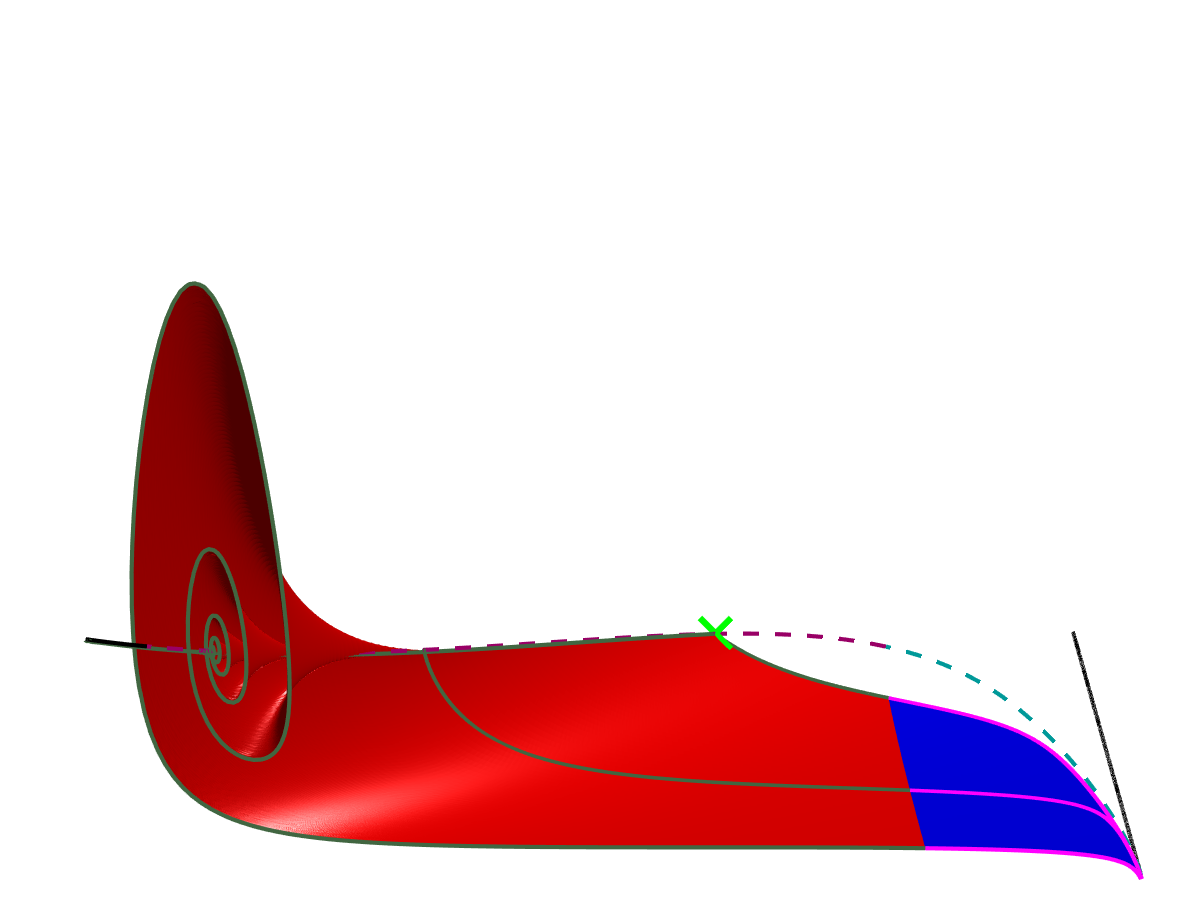
\includegraphics[width=12.6cm]{./figures_raw/hetclin_6_BAY.eps}}
	    \put(92.5,32){$\mathscr{L}$}
	    \put(90,22.5){$C^2$}
	    \put(106,13){$C^3$}
	    \put(108,6.5){$C^{4}_{+}$}
	    \put(2.5,42){$C^{4}_{-}$}
	    \put(48,3){$\mathscr{H}$}
	    \put(6.75,34.5){$H$}
	    \put(79,26.5){$q$}
	    \put(99,20.5){$F_2$}
	    \put(91,-0.5){$F_1$}
	    \put(5,81){(b)}
	\end{picture}
	\caption{}
}
\end{picture}
\end{figure}
\newpage

%%%%%%%%%%%%%%%%%%%%%%%%%%%%%%%%%%%
%% Figure 10: Faded heteroclinic surface with unstable manifold %%
%%%%%%%%%%%%%%%%%%%%%%%%%%%%%%%%%%%

\begin{figure}
\begin{picture}(124,175)(51,69.5)
\put(50,162){
	\begin{picture}(180,100)(0,0)
	    \put(0,0){\includegraphics[width=12.6cm]{./figures_raw/paper_saddle_unstable_BAX.eps}}
	    \put(91,72){$W^u(q)$}
	    \put(105.5,28){$C^3$}
	    \put(108,4.5){$C^{4}_{+}$}
	    \put(91,-1){$F_1$}
	     \put(2.5,54.5){$C^{4}_{-}$}
	      \put(6.75,48){$H$}
	     \put(48,7){$\mathscr{H}$}
	     \put(81,43.5){$q$}
	    \put(5,77){(a)}
	\end{picture}
	\caption{}
}

\put(50,71.5){
	\begin{picture}(180,100)(0,0)
	    \put(0,0){\includegraphics[width=12.6cm]{./figures_raw/paper_saddle_unstable_BAY.eps}}
	    \put(87,51){$W^u(q)$}
	    \put(105.5,13){$C^3$}
	    \put(108,4.5){$C^{4}_{+}$}
	    \put(2.5,41.5){$C^{4}_{-}$}
	    \put(6.75,34){$H$}
	    \put(48,1.5){$\mathscr{H}$}
	    \put(91,-1){$F_1$}
	    \put(81,23){$q$}
	    \put(5,81){(b)}
	\end{picture}
	\caption{}
}
\end{picture}
\end{figure}
\newpage

%%%%%%%%%%%%%%%%%%%%%%%%%%%%%%%%%%%%%
%% Figure 11: Compare non-singular with singular heteroclinic surface %%
%%%%%%%%%%%%%%%%%%%%%%%%%%%%%%%%%%%%%

\begin{figure}
\begin{picture}(124,169)(51,53)
\put(50,140){
	\begin{picture}(180,100)(0,0)
	    \put(0,0){\includegraphics[width=12.6cm]{./figures_raw/paper_BAX.eps}}
	    \put(90,41){$C^2$}
	     \put(81.5,45){$q$}
	    \put(105.5,28){$C^3$}
	    \put(99.5,37.5){$F_2$}
	    \put(108,4.5){$C^{4}_{+}$}
	    \put(91,-1){$F_1$}
	     \put(2.5,54.5){$C^{4}_{-}$}
	      \put(6.75,48){$H$}
	     \put(48,7){$\mathscr{H}$}
	    \put(5,77){(a)}
	\end{picture}
	\caption{}
}

\put(50,55){
	\begin{picture}(180,100)(0,0)
	    \put(0,0){\includegraphics[width=12.6cm]{./figures_raw/paper_singular_BAX.eps}}
 \put(90,41){$C^2$}
	     \put(81.5,45){$q$}
	    \put(105.5,28){$C^3$}
	    \put(99.5,37.5){$F_2$}
	    \put(108,4.5){$C^{4}_{+}$}
	    \put(91,-1){$F_1$}
	     \put(2.5,54.5){$C^{4}_{-}$}
	      \put(6.75,48){$H$}
	     \put(48,7){$\mathscr{H}_0$}
	    \put(5,81){(b)}
	\end{picture}
	\caption{}
}
\end{picture}
\end{figure}
\newpage

%%%%%%%%%%%%%%%%%%%
%%%% Figure 12: Isola figure %%%
%%%%%%%%%%%%%%%%%%%

\begin{figure}
	\begin{picture}(124,64.5)(86.5,96.5)
	    \put(100,100){\includegraphics[width=11cm]{./figures_raw/paper_isola.eps}}
	    \put(87,157){max($A$)}
	    \put(94,139){\footnotesize $9.75$}
	    \put(94,119){\footnotesize $7.25$}
            \put(207,96.75){\Large $\varepsilon$}
            \put(120.5,97){\footnotesize$0.3$}
            \put(144.5,97){\footnotesize$0.5$}
            \put(167.5,97){\footnotesize$0.7$}
            \put(190.5,97){\footnotesize$0.9$}
            \put(194,149.5){(a)}
            \put(104,138){(b)}
            \put(196.5,110){(c)}
            
	\end{picture}
	\caption{}
\end{figure}

\newpage

%%%%%%%%%%%%%%%%%%%%%%%%%
%%%% Figure 13: MMO surface interaction %%%
%%%%%%%%%%%%%%%%%%%%%%%%%

\begin{figure}
\begin{picture}(107,93)(64,137.5)
\put(50,140){
	\begin{picture}(180,100)(0,0)
	    \put(0,0){\includegraphics[width=12.6cm]{./figures_raw/MMO_surface_interaction_BAX.eps}}
	    \put(114,13.25){$C^2$}
	    \put(107,4){$C^3$}
	    \put(108,81){(b)}
	    \put(95,42){$\mathscr{H}$}
	    \put(65,-1){$C^{4}_{+}$}
	    \put(16,1){$F_1$}
	    \put(20,17.5){$C^{4}_{-}$}
	    \put(80,19){$\mathscr{H}$}
	    \put(14,50){$\Gamma$}
	    \put(13,81){(a)}
	    \put(115.5,8){$F_2$}
	\end{picture}
	\caption{}
}
\end{picture}
\end{figure}
\newpage

%%%%%%%%%%%%%%%%%%%%%%%%%%%%%%%%%%%%%
%% Figure 14: Compare MMOs and singular objects%%
%%%%%%%%%%%%%%%%%%%%%%%%%%%%%%%%%%%%%

\begin{figure}
\begin{picture}(160,192)(76,81)


\put(50,163){
	\begin{picture}(180,100)(0,0)
	    \put(0,0){\includegraphics[width=12.6cm]{./figures_raw/MMO_2_BAX.eps}}
	    \put(70,-2){$C^{4}_{+}$}
	     \put(26,16){$C^{4}_{-}$}
	     \put(90,18){$\mathscr{H}_0$}
	     \put(65,50){$\mathscr{P}$}
	     \put(56,40){$\Gamma$}
	     \put(34,49){$\mathscr{J}$}
	     \put(105.5,17.5){$\mathscr{J}^*$}
	     \put(33,-1){$F_1$}
	    \put(25,60){(b)}
	\end{picture}
	\caption{}
}

\put(120,199){
	\begin{picture}(180,100)(0,0)
	    \put(0,0){\includegraphics[width=12.6cm]{./figures_raw/MMO_1_BAX.eps}}
	    \put(70,-2){$C^{4}_{+}$}
	     \put(26,16){$C^{4}_{-}$}
	     \put(90,18){$\mathscr{H}_0$}
	     \put(64,50){$\mathscr{P}$}
	     \put(24.5,40){$\Gamma$}
	     \put(34,49){$\mathscr{J}$}
	     \put(105.5,17.5){$\mathscr{J}^*$}
	     \put(33,-1){$F_1$}
	    \put(25,60){(a)}
	\end{picture}
	\caption{}
}

\put(120,85){
	\begin{picture}(180,100)(0,0)
	    \put(0,0){\includegraphics[width=12.6cm]{./figures_raw/MMO_3_BAX.eps}}
	    \put(70,-2){$C^{4}_{+}$}
	     \put(26,16){$C^{4}_{-}$}
	     \put(90,18){$\mathscr{H}_0$}
	     \put(64,50){$\mathscr{P}$}
	     \put(25,40){$\Gamma$}
	     \put(34,49){$\mathscr{J}$}
	     \put(105.5,17.5){$\mathscr{J}^*$}
	     \put(33,-1){$F_1$}
	    \put(25,60){(c)}
	\end{picture}
	\caption{}
}

\end{picture}
\end{figure}
\newpage

\end{document}
